\chapter{Advanced Sample Selection}
\ifpdf
    \graphicspath{{Chapter3/Chapter3Figs/PNG/}{Chapter3/Chapter3Figs/PDF/}{Chapter3/Chapter3Figs/}}
\else
    \graphicspath{{Chapter3/Chapter3Figs/EPS/}{Chapter3/Chapter3Figs/}}
\fi


Now that we have a good idea of what active sampling involves attention will be focused to more advanced algorithms with the aim of improving performance.
\section{Clustered Knowledge Sampling}
\label{sec:cks}
\markboth{\MakeUppercase{\thechapter. Advanced Sample Selection }}{\thechapter. Advanced Sample Selection}
In the proposed minimum knowledge search algorithm (section \ref{sec:mks_alg}), its poor performance was mainly due to ignoring the data and only focusing on the mask matrix, which homogenised the amount of known samples. This had two problems, one in situations with search space constraints and the other for actually ignoring data and not taking "information" into account.


\subsection{Outline}

\begin{figure}[!htbp]
  \begin{center}
    \resizebox{\textwidth}{!}{% This file was created by matlab2tikz v0.4.7 running on MATLAB 8.1.
% Copyright (c) 2008--2014, Nico Schlömer <nico.schloemer@gmail.com>
% All rights reserved.
% Minimal pgfplots version: 1.3
% 
% The latest updates can be retrieved from
%   http://www.mathworks.com/matlabcentral/fileexchange/22022-matlab2tikz
% where you can also make suggestions and rate matlab2tikz.
% 
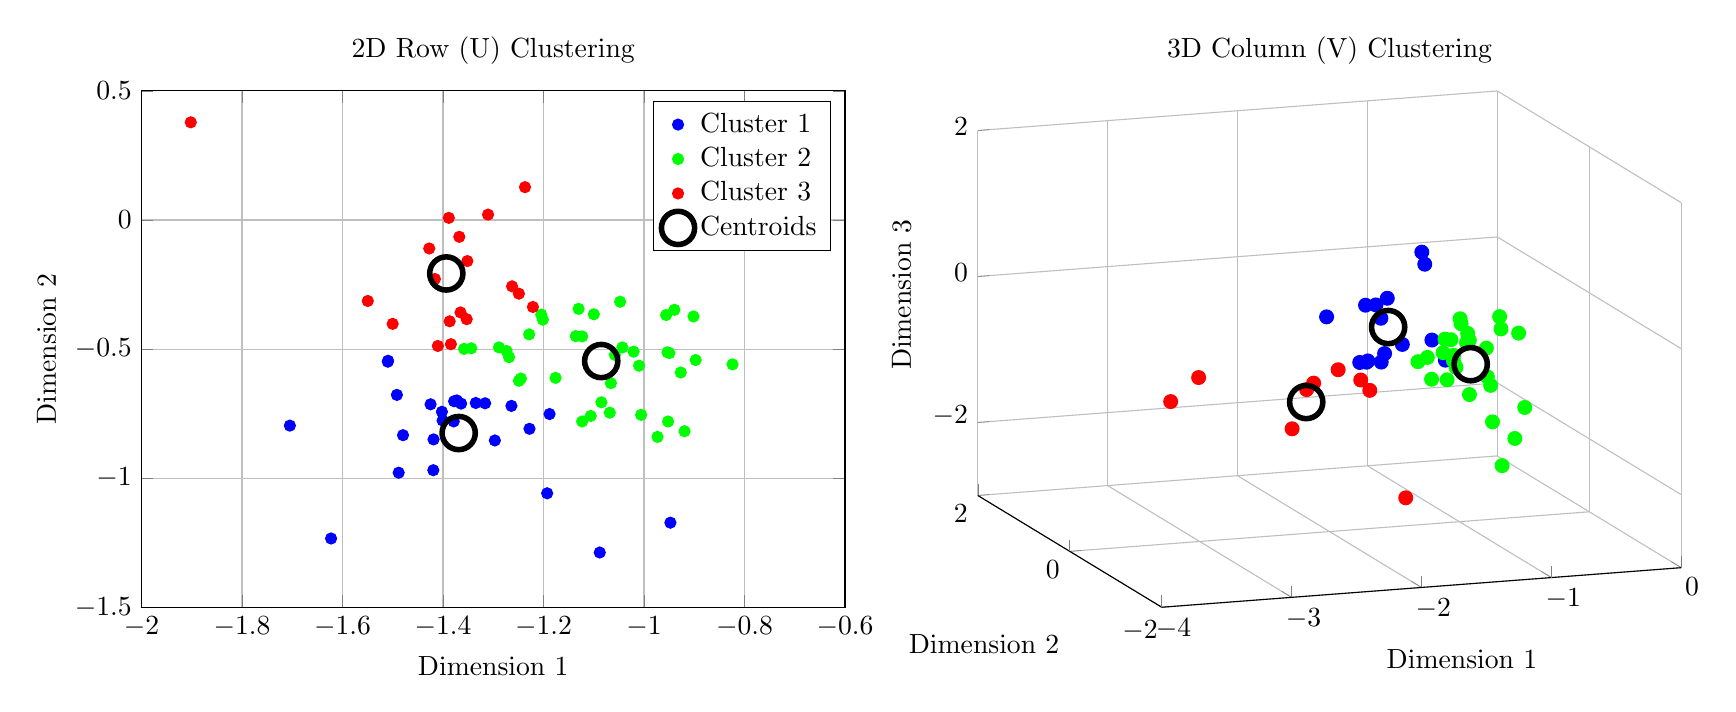
\begin{tikzpicture}

\begin{axis}[%
width=3.51740648674242in,
height=2.58151041666667in,
view={-19.5}{18},
scale only axis,
xmin=-4,
xmax=0,
xlabel={Dimension 1},
xmajorgrids,
ymin=-2,
ymax=2,
ylabel={Dimension 2},
ymajorgrids,
zmin=-3,
zmax=2,
zlabel={Dimension 3},
zmajorgrids,
name=plot1,
title={3D Column (V) Clustering},
axis x line*=bottom,
axis y line*=left,
axis z line*=left
]
\addplot3 [color=blue,mark size=2.5pt,only marks,mark=*,mark options={solid}]
 table[row sep=crcr] {-1.59044540063681	0.148396996168405	-0.00698558731390522\\
-1.86602726252353	-0.404299596558771	0.238047600835955\\
-2.15402023110266	-0.370963692226637	0.104703420377893\\
-2.01836370251589	-0.708482579480979	-0.409582767022601\\
-1.3601021205625	-0.263476524470756	0.677007101878209\\
-1.84863640992759	-0.405737385391855	-0.527296075866767\\
-1.8297149862398	-0.635270366202015	0.142259654037909\\
-1.85319119891177	-1.591979484085	1.4180250028355\\
-1.53407932701679	-1.2029284069621	-0.254406365200206\\
-1.96308377629313	-1.02005617297288	-0.292600342652495\\
-1.4800140593837	-0.757826699388731	-0.156283097895312\\
-1.98325658275392	-1.14987990275354	-0.123521101234678\\
-2.0902575666433	-1.06113716256017	-0.261223194073795\\
-1.6044250712648	-0.138809835184553	0.196026800172275\\
-1.79360406022386	-1.00024498034514	-0.0808198205638491\\
};
 \addplot3 [color=green,mark size=2.5pt,only marks,mark=*,mark options={solid}]
 table[row sep=crcr] {-1.47671051242454	-0.740544172774373	-0.700265880452768\\
-0.93252978607874	-0.737858573994506	-1.95864940281495\\
-1.39095127404548	-1.03082252266447	-0.436930323751058\\
-0.826190098315246	-0.796788433464611	-0.135195116811069\\
-1.14564673815213	-0.226979187418543	-0.400313692051324\\
-1.28640712006202	-0.454245485913808	-0.471703201832827\\
-1.07636956454563	-0.823100337923473	-0.689844042349405\\
-1.12469679933646	-0.389700844325155	-0.123064999816717\\
-1.09992565114399	-0.498384325340187	-0.31048726329556\\
-1.41309679459476	-1.38500223790909	-0.671990025552719\\
-1.25556262289311	-0.595096473274391	-0.458811626470363\\
-1.38017147536982	-0.806158272944827	-0.696454758506215\\
-1.1184806298713	-1.755123688963	-0.747224784979808\\
-1.0831580755134	-0.820895730212531	-0.296258382112644\\
-1.48188468231259	-0.460624191506098	-0.566309707097411\\
-1.11563748443596	-1.00507440936161	-0.732314861859024\\
-0.929163965552316	-0.519647699876556	-1.44361838242822\\
-1.19434558073037	-0.703961212433198	-0.251105760079353\\
-1.46380901634084	-0.611874379533737	-0.452599705977574\\
-1.31478254435664	-0.575143613118262	-0.236189435731263\\
-1.09688073201687	-0.289096106073911	-0.0960876831079487\\
-0.773050817612426	-0.233815087553789	-0.131884904110039\\
-0.813338320663528	-0.377167666478255	-0.24029048766129\\
-0.876771344375913	-0.857072651175691	-1.54870993973188\\
-1.14990983972071	-0.29358421798426	-0.663112219132381\\
-1.13003602840388	-0.546883342757847	-0.193711899583056\\
};
 \addplot3 [color=red,mark size=2.5pt,only marks,mark=*,mark options={solid}]
 table[row sep=crcr] {-2.11607881604296	-1.20309665474736	-0.589023084252537\\
-2.35807960849134	-1.19898464092221	-0.275036292209193\\
-2.45276407893644	-0.465205348869312	-1.35246640183301\\
-1.85926734892307	-1.25963112352855	-2.07438098640639\\
-3.47098887962986	-0.700065408270514	-0.751679331712361\\
-2.21876190776304	-1.29614469556361	-0.397752621498269\\
-2.47690496220663	-1.00083546374682	-0.518829309125334\\
-2.45427807746748	-0.78414820561212	-0.692778019848313\\
-3.4342351998618	-1.2039455085677	-0.234307040855988\\
};
 \addplot3 [color=black,line width=2.0pt,mark size=6.0pt,only marks,mark=o,mark options={solid}]
 table[row sep=crcr] {-1.79794811706667	-0.704179719494315	0.0442234152209426\\
-1.15190413457187	-0.674409417883699	-0.563581864896033\\
-2.53792876436918	-1.01245078331424	-0.765139231971266\\
};
 \end{axis}

\begin{axis}[%
width=3.51740648674242in,
height=2.58151041666667in,
scale only axis,
xmin=-2,
xmax=-0.6,
xlabel={Dimension 1},
xmajorgrids,
ymin=-1.5,
ymax=0.5,
ylabel={Dimension 2},
ymajorgrids,
at=(plot1.left of south west),
anchor=right of south east,
title={2D Row (U) Clustering},
legend style={draw=black,fill=white,legend cell align=left}
]
\addplot [color=blue,mark size=2.0pt,only marks,mark=*,mark options={solid}]
  table[row sep=crcr]{-0.947397094097976	-1.17240232446132\\
-1.42464042756946	-0.713815591075102\\
-1.22781208226467	-0.808765943560055\\
-1.37238484821147	-0.698803283515191\\
-1.37781059027466	-0.702054360358239\\
-1.08796797285841	-1.28792997752542\\
-1.41920362072619	-0.969141960295007\\
-1.49169444482093	-0.67739390245747\\
-1.26374363723324	-0.720049936258417\\
-1.33466016547064	-0.708718593754529\\
-1.48811954757637	-0.9788217818583\\
-1.1878838257152	-0.751578697212706\\
-1.36389755394777	-0.711223029487005\\
-1.50926630817321	-0.545099702809181\\
-1.40069149027704	-0.776586360666373\\
-1.50975621361547	-0.548801346804066\\
-1.37855408387926	-0.780159670397303\\
-1.31611978200492	-0.709930659849702\\
-1.418751280377	-0.849795612755271\\
-1.19267570375899	-1.05856633692692\\
-1.47951050417601	-0.833441522749927\\
-1.40210224009503	-0.742883948823392\\
-1.70466946988011	-0.796421429139088\\
-1.62266369930196	-1.23367702017733\\
-1.29673298795604	-0.853960506960763\\
};
\addlegendentry{Cluster 1};

\addplot [color=green,only marks,mark=*,mark options={solid}]
  table[row sep=crcr]{-0.952004639322655	-0.780407744162834\\
-1.35800804056431	-0.499095126768185\\
-1.12301132961619	-0.450813783470718\\
-1.06803088855719	-0.746252586925583\\
-1.04742072820829	-0.316512594208732\\
-1.00563006266044	-0.754667394539394\\
-1.08471290104999	-0.706052703408371\\
-0.972986130578649	-0.840038953765678\\
-0.926768452677666	-0.590670764290693\\
-1.10598706869137	-0.759020761417815\\
-1.12299454549838	-0.780455778963848\\
-1.34375616408669	-0.496931240615796\\
-0.823701319540284	-0.55922528432968\\
-1.27345811398	-0.506983755622736\\
-1.05784721496967	-0.52241729560441\\
-0.949405224340586	-0.515403391466322\\
-1.00973566569467	-0.564270108492813\\
-0.897178142840313	-0.542394334642152\\
-1.28850500158151	-0.493491662522362\\
-1.20120133077088	-0.385865901893781\\
-1.13005221396697	-0.344149415912444\\
-1.22851393427091	-0.442937560581115\\
-1.26844999472948	-0.531171960691112\\
-1.09980175514811	-0.365281432703934\\
-0.901446106339055	-0.373594412602389\\
-1.24886587648314	-0.622710283455377\\
-0.955827125951069	-0.368068581593385\\
-0.919233297957232	-0.818242177080642\\
-1.02058986705701	-0.509959799649133\\
-1.20447547808101	-0.36632574209671\\
-0.939403310754379	-0.347838228723723\\
-1.06577253942638	-0.631933383632939\\
-1.13563758881092	-0.449750374425283\\
-1.17592385721954	-0.611327813248462\\
-0.953229779684915	-0.512455651100702\\
-1.04297625053534	-0.493442994365538\\
-1.24488239946148	-0.61392004639489\\
};
\addlegendentry{Cluster 2};

\addplot [color=red,only marks,mark=*,mark options={solid}]
  table[row sep=crcr]{-1.38667570143095	-0.392327756779921\\
-1.90191402108737	0.37843174742415\\
-1.35145177681762	-0.159014906937421\\
-1.38834556565347	0.00828026112936182\\
-1.42731217565679	-0.110223842769362\\
-1.50012813166991	-0.402262676901485\\
-1.23673403705109	0.127286862615916\\
-1.54961317850779	-0.313606751908253\\
-1.38424609474405	-0.480950419640141\\
-1.41015507760762	-0.487840276904245\\
-1.31029966299755	0.0210377007725251\\
-1.3650626694132	-0.358014675162437\\
-1.35275033416153	-0.384139741274205\\
-1.24893755013947	-0.285353484220869\\
-1.22099935349909	-0.336870067395305\\
-1.36748608818927	-0.0650839050816374\\
-1.41608032676241	-0.228524593438377\\
-1.26244189537061	-0.256869879155967\\
};
\addlegendentry{Cluster 3};

\addplot [color=black,line width=2.0pt,mark size=6.0pt,only marks,mark=o,mark options={solid}]
  table[row sep=crcr]{-1.36874838297048	-0.825200939995123\\
-1.08506552273261	-0.54632651419918\\
-1.39336853559777	-0.207002578090426\\
};
\addlegendentry{Centroids};

\end{axis}
\end{tikzpicture}%}
  \end{center}
    
$U$ and $V$ from synthetic dataset with 15\% of samples initially discovered.  $\lambda = 0.01$, $D=7$

Dimensions reduced for plotting purposes
    \caption{Sample k-means clustering of U and V by features}
    \label{fig:u_v_cluster}
\end{figure}

Minimum knowledge search failed to integrate information about the known data to target more informative samples. Here we decide to take advantage of the $U$ and $V$ matrices formed during matrix factorisation , as in equation \ref{eq:rsimeq}. Each of the columns of $U$ and $V$ are supposed to represent features of the related row or column. We now assume that if we knew a minimal amount of each feature it will be possible to cluster rows and columns into groups. Figure \ref{fig:u_v_cluster} shows the features of U and V clustered into 3 different groups\footnote{3 was arbitrarily chosen as the number of clusters}. In the case of drug-target interaction database dimension 1 could represent the estimated presence of a chemical, say $H_2O$ and the second dimension of the presence that represents the presence of another chemical.

In collaborative filtering we seek to infer these features to best reconstruct the full matrix. The idea behind clustered sample selection is to target the groups with the least certainty, to improve their accuracy and the model as a whole. In a movie-user scenario this means that we can separate the thriller film liking users from the drama movie liking users, then if we find out that less is know on thriller liking people then the model should be better off learning an extra datapoint on that group. This would allow for row selection and the selection of columns can be done in a similar way. We will define knowledge in the same way as minimum knowledge search, as the fraction of known rows and columns.



\subsection{Algorithm}

We base the work of the clustered knowledge search on the minimum knowledge search algorithm, in that we will target not the specfic row-column combination we know less about but the row-colum cluster we know the less about. 

The first step involves determining the ideal number of clusters for a dataset. In itself this is not an easy task and can increase algorithm complexity due to having to test for all different candidate number of clusters. To determine the number of clusters we use the silhouette measure \cite{kmean-sil} which essentially measures how tight data is when in a group. It is not always effective but does the job. 
%Explain how to cluster in silhoutettes



\begin{algorithm}
\caption{Clustered Knowledge Search algorithm}\label{alg:cks}
\begin{algorithmic}[1]
\Procedure{ClusKnowSearch}{$U$,$V$,$Z$}
\State $k_U \gets \text{NumOfClust}(U)$ \Comment{Returns best guess of number of clusters}
\State $k_V \gets \text{NumOfClust}(V)$
\State $u_{\text{clusters}} = \text{kmeans}(U,k_U)$ \Comment{Assigns cluster IDs}
\State $v_{\text{clusters}} = \text{kmeans}(V,k_V)$
\State $\mathbf{u_{info}} \gets \text{meanrow}(Z)$ \Comment{$\in \mathbb{R}^N$}
\State $\mathbf{v_{info}} \gets \text{meancol}(Z)$ \Comment{$\in \mathbb{R}^M$}
\State $\mathbf{a} \gets \mathbf{0}^{N}$ \Comment{$\in \mathbb{R}^N$}
\State $\mathbf{b} \gets \mathbf{0}^{M}$ \Comment{$\in \mathbb{R}^M$}
\For{$i=1\dots k_U$}
\State $\mathbf{u_{knowl}}[i] \gets \sum\limits_{\text{index}=i} \mathbf{u_{info}}$ \Comment{Adds up all info values}
\State $\mathbf{a}[{index\; u_{\text{clusters}} =i}] = \mathbf{u_{knowl}}[i]$ \Comment{Assigns sum of info to clusters}
\EndFor

\For{$j=1\dots k_V$}
\State $\mathbf{v_{knowl}}[j] \gets \sum\limits_{\text{index}=j} \mathbf{v_{info}}$
\State $\mathbf{b}[{index\; v_{\text{clusters}} =j}] = \mathbf{v_{knowl}}[j]$
\EndFor

\State $K \gets \mathbf{a}^T \cdot \mathbf{b}$ \Comment{ $K \in \mathbb{R}^{M\times N}$}
\State $x,y \gets index\_of\_min(K)$ \Comment{Many candidates, one is chosen at random} \label{alg:line:select}
\While{$x,y$ not valid sample request}
\State $x,y \gets next\_min\_index(K)$
\EndWhile
\State \textbf{return} $x,y$\Comment{Return $x,y$ that has least knowledge}
\EndProcedure
\end{algorithmic}
\end{algorithm}

Once we have determined the number of clusters, we cluster the rows and columns according to the features of $U$ and $V$ using a clustering algorithm. K-means was chosen for being fast yet good at clustering. Alternatives such as GMM were considered but found to not be appropriate due to their great increase in complexity and little increase in clustering quality.

\nomenclature{GMM}{Gaussian Mixture Model - A probabilistic model for representing the presence of subsets within an overall dataset}

\nomenclature{K-Means}{K-Means Clustering - A popular algorithm for cluster analysis, which separates $N$ data points into $K$ clusters around centroids}


From the clustered rows we create the vectors $\mathbf{a}$ and $\mathbf{b}$ which contain the amount know of each cluster. This allows the create of the knowledge matrix, $K =\mathbf{a}^T \cdot \mathbf{b}$. From this a sample is selected as in section \ref{sec:mks_alg}.

This algorithm is defined formally in algorithm \ref{alg:cks}.
%\subsubsection{Clustering observations}
%... and some more in the first subsub section otherwise it all looks the same
%doesn't it? well we can add some text to it ...

\subsection{Performance}
The first initial observations on the performance is that during a cold-start, that is when very little is know about the matrix, clustering will not perform well and sample selection will effectively be random. As soon as enough data is gathered a large advantage compared to random sampling is usually observed. This is because, unlike the minimum knowledge search, the search area is always restricted to a reasonably small subset.


It will also tend to cluster currently unknown groups of data together and targeting them even later on in execution which is useful. However once the number of unknown rows and columns have fallen down it suffers from not requesting individual rows and columns with no knowledge if they are assigned to a cluster of high information - this seemed to be the main drawback from this algorithm. This can be seen from the lines in figure \ref{fig:eiffel_clustering_random} which are never requested. This is why it is preferred to randomly sample from the restricted subset (line \ref{alg:line:select} in algorithm \ref{alg:cks}) as it can mitigate this problem. In cases where the first available value of the subset is selected, the algorithm was found to sometimes perform worse than random in very late stages, due to removing the ability to sample from certain, useful, areas.



\begin{figure}[!htbp]
  \begin{center}
    \resizebox{\textwidth}{!}{% This file was created by matlab2tikz v0.4.7 running on MATLAB 8.1.
% Copyright (c) 2008--2014, Nico Schlömer <nico.schloemer@gmail.com>
% All rights reserved.
% Minimal pgfplots version: 1.3
% 
% The latest updates can be retrieved from
%   http://www.mathworks.com/matlabcentral/fileexchange/22022-matlab2tikz
% where you can also make suggestions and rate matlab2tikz.
% 
\begin{tikzpicture}

\begin{axis}[%
width=1.67990913120567in,
height=2.06885416666667in,
axis on top,
scale only axis,
xmin=0.5,
xmax=50.5,
y dir=reverse,
ymin=0.5,
ymax=80.5,
name=plot2,
title={Targeted RMSE:0.806}
]
\addplot [forget plot] graphics [xmin=0.5,xmax=50.5,ymin=0.5,ymax=80.5] {eiffel_clustering_random-1.png};
\end{axis}

\begin{axis}[%
width=1.67990913120567in,
height=2.06885416666667in,
axis on top,
scale only axis,
xmin=0.5,
xmax=50.5,
y dir=reverse,
ymin=0.5,
ymax=80.5,
at=(plot2.left of south west),
anchor=right of south east,
title={Random RMSE:0.839}
]
\addplot [forget plot] graphics [xmin=0.5,xmax=50.5,ymin=0.5,ymax=80.5] {eiffel_clustering_random-2.png};
\end{axis}

\begin{axis}[%
width=1.67990913120567in,
height=2.06885416666667in,
scale only axis,
xmin=0,
xmax=1000,
xlabel={Discovered Samples},
xmajorgrids,
ymin=0.5,
ymax=3.5,
ylabel={RMSE},
ymajorgrids,
name=plot3,
at=(plot2.right of south east),
anchor=left of south west,
title={Target Advantage:1.033}
]
\addplot [color=blue,solid,forget plot]
  table[row sep=crcr]{1	3.23608821969601\\
4	3.23874456682935\\
7	3.23400303366272\\
10	3.22686273151906\\
13	3.22064145645356\\
16	3.210065518808\\
19	3.20609812591828\\
22	3.20094180016412\\
25	3.19290280170711\\
28	3.18218381413051\\
31	3.16964031933361\\
34	3.1683939149483\\
37	3.14902695809985\\
40	3.14063222906248\\
43	3.13273566512044\\
46	3.13792693466917\\
49	3.13819075795978\\
52	3.13919418631302\\
55	3.12774596457256\\
58	3.10462488420985\\
61	3.08908746474799\\
64	3.06099903675343\\
67	3.03884916723113\\
70	2.99517372420138\\
73	2.97196825627754\\
76	2.97256611010417\\
79	2.95382968686519\\
82	2.95634785166779\\
85	2.94868953281047\\
88	2.94325789737375\\
91	2.94350848161074\\
94	2.91336774342895\\
97	2.90056982311092\\
100	2.85923501691438\\
103	2.83740090301335\\
106	2.79845083538125\\
109	2.77376523447295\\
112	2.75413976151122\\
115	2.74400949224298\\
118	2.70028004286642\\
121	2.67358627982908\\
124	2.62618230680027\\
127	2.5991518051474\\
130	2.56216884913842\\
133	2.50799167659206\\
136	2.50385337795266\\
139	2.4803382802154\\
142	2.44636183251382\\
145	2.41592726658385\\
148	2.39933224583661\\
151	2.40277511320256\\
154	2.34731779980291\\
157	2.3070855826964\\
160	2.2896257555724\\
163	2.23026298414911\\
166	2.21708749193983\\
169	2.17344338947626\\
172	2.13681549115793\\
175	2.13195859805556\\
178	2.08980570866445\\
181	2.07051216580413\\
184	2.0290780770062\\
187	2.00290502932381\\
190	1.97208451698914\\
193	1.94062234122199\\
196	1.91740161345952\\
199	1.87986542638094\\
202	1.84671693422685\\
205	1.82186129157887\\
208	1.79450537588702\\
211	1.76763352842766\\
214	1.74168676243316\\
217	1.72430216808774\\
220	1.71889477376259\\
223	1.68961112331644\\
226	1.67025781087249\\
229	1.65326196179016\\
232	1.60945972087621\\
235	1.58258047471896\\
238	1.54487313115169\\
241	1.51817513386755\\
244	1.49070521269874\\
247	1.46080281702285\\
250	1.44720905111535\\
253	1.43926025170762\\
256	1.40292904023112\\
259	1.38659439540347\\
262	1.37895909165236\\
265	1.35672297317994\\
268	1.35092785676313\\
271	1.33117400480906\\
274	1.33258414460804\\
277	1.3253190477257\\
280	1.31368167800342\\
283	1.29119318682901\\
286	1.2847957937692\\
289	1.26668265767296\\
292	1.24925263988163\\
295	1.22933860498004\\
298	1.22269200109639\\
301	1.217588049285\\
304	1.20608664660767\\
307	1.19807300208598\\
310	1.19758312124881\\
313	1.1938256302761\\
316	1.18716489873387\\
319	1.19029671808817\\
322	1.18292779724569\\
325	1.17282069844146\\
328	1.15851505986828\\
331	1.15456764680907\\
334	1.14508764016097\\
337	1.12668385447176\\
340	1.11143941981602\\
343	1.10514593946996\\
346	1.10304784064215\\
349	1.10116816111664\\
352	1.09107633565513\\
355	1.08633596051687\\
358	1.08516499819841\\
361	1.07959210657411\\
364	1.07530032022216\\
367	1.07216539510789\\
370	1.06622687994884\\
373	1.06630297628754\\
376	1.06260705350293\\
379	1.06175827182202\\
382	1.06143183296372\\
385	1.05791649140148\\
388	1.05409250877161\\
391	1.05161336131875\\
394	1.05116623420654\\
397	1.05016516103723\\
400	1.04877986780112\\
403	1.04630129440592\\
406	1.04418511076514\\
409	1.04450441148256\\
412	1.0411350617253\\
415	1.04074781344838\\
418	1.04105816040508\\
421	1.03891783350241\\
424	1.03846898033468\\
427	1.03366056108131\\
430	1.0349054643268\\
433	1.03293572208455\\
436	1.02914529258533\\
439	1.02837604894394\\
442	1.02288217203224\\
445	1.01917734623858\\
448	1.01660529190564\\
451	1.01104633503953\\
454	1.00738780460553\\
457	1.00472484329262\\
460	1.0039520994342\\
463	1.00523368157343\\
466	1.0034014855957\\
469	1.00115415201671\\
472	1.00131717115537\\
475	1.00140154452006\\
478	0.999600501577712\\
481	0.997030854659885\\
484	0.996596829338407\\
487	0.998956506591063\\
490	0.996396119941576\\
493	0.99678747484711\\
496	0.995812517884907\\
499	0.996549742510299\\
502	0.997814025890126\\
505	0.997465160219533\\
508	0.998205183905975\\
511	0.996700572212048\\
514	0.992192014135254\\
517	0.99017274589718\\
520	0.988246220181901\\
523	0.983527543116826\\
526	0.980158352527665\\
529	0.976936631596359\\
532	0.973841590288914\\
535	0.971683759345203\\
538	0.97021998537905\\
541	0.970087303017605\\
544	0.966875404562843\\
547	0.965446355399993\\
550	0.961156860324029\\
553	0.960736860199741\\
556	0.959573196397698\\
559	0.958172455028803\\
562	0.958770783614183\\
565	0.95942333309407\\
568	0.95675523315015\\
571	0.954985652638341\\
574	0.953754982262894\\
577	0.951951640394101\\
580	0.950033484240326\\
583	0.947777327611643\\
586	0.944826363270912\\
589	0.944952886290964\\
592	0.94315558643634\\
595	0.941699990458453\\
598	0.938536696327822\\
601	0.937049163550473\\
604	0.936679555970613\\
607	0.936292576650164\\
610	0.934670013600377\\
613	0.933201096489967\\
616	0.932154862665519\\
619	0.935070401434189\\
622	0.935818514423071\\
625	0.934527979357141\\
628	0.934906714264051\\
631	0.935615129794311\\
634	0.936366242579699\\
637	0.935284780247618\\
640	0.932280549739419\\
643	0.931216722723593\\
646	0.930150141619051\\
649	0.928546240457424\\
652	0.925445991397538\\
655	0.92497766091949\\
658	0.92524494521337\\
661	0.925938557632788\\
664	0.921872445167552\\
667	0.922655597972024\\
670	0.926914387150573\\
673	0.923358707406725\\
676	0.918656594203506\\
679	0.923113626000366\\
682	0.923673712709766\\
685	0.923765488220372\\
688	0.925829658005833\\
691	0.928196910759219\\
694	0.930349324771632\\
697	0.930915786574827\\
700	0.928988500185951\\
703	0.931445992770396\\
706	0.931045664349461\\
709	0.930085759627698\\
712	0.927684194495509\\
715	0.924206707903442\\
718	0.917216929973831\\
721	0.9138815695211\\
724	0.910281899990097\\
727	0.9048235024033\\
730	0.901690576891687\\
733	0.901556019448105\\
736	0.901076836371851\\
739	0.898997400601895\\
742	0.898609734264734\\
745	0.898487285087361\\
748	0.896874150045249\\
751	0.896184674262905\\
754	0.89464558708581\\
757	0.89371816401248\\
760	0.891675939489928\\
763	0.889270954104735\\
766	0.887393356920999\\
769	0.888966477789644\\
772	0.889796743924115\\
775	0.889217325274594\\
778	0.886175970567902\\
781	0.887831673635639\\
784	0.884393887310554\\
787	0.881405784230714\\
790	0.875125770607302\\
793	0.875491739240181\\
796	0.873320815865276\\
799	0.872607897223783\\
802	0.871275216169282\\
805	0.870729415201652\\
808	0.868897845035715\\
811	0.867814864589322\\
814	0.865641713524941\\
817	0.867104401643685\\
820	0.864460449379786\\
823	0.865104730667196\\
826	0.864160878179792\\
829	0.864625887542073\\
832	0.863328213106487\\
835	0.860767751860216\\
838	0.859966998307642\\
841	0.857019519810177\\
844	0.857987718098942\\
847	0.856739782088524\\
850	0.856577326039197\\
853	0.856560098757885\\
856	0.854184426682648\\
859	0.85348915660362\\
862	0.851685450224478\\
865	0.848851766170523\\
868	0.849928253030711\\
871	0.851961364717722\\
874	0.853659193033011\\
877	0.856835734709883\\
880	0.859220693886935\\
883	0.863043394077267\\
886	0.865315484430734\\
889	0.866086515663051\\
892	0.867300737937679\\
895	0.868230565044493\\
898	0.868322860414097\\
901	0.86568408442662\\
904	0.861998055926054\\
907	0.86052347090935\\
910	0.859925430757205\\
913	0.858086205182545\\
916	0.857451962604108\\
919	0.856321452316256\\
922	0.858089207726632\\
925	0.856844921576297\\
928	0.853638586216406\\
931	0.85396213461611\\
934	0.852728595458033\\
937	0.851397625110357\\
940	0.852107411623177\\
943	0.852585438816453\\
946	0.853087631098825\\
949	0.853034693501791\\
952	0.851691813071311\\
955	0.850075931017224\\
958	0.849901912244008\\
961	0.85075354738233\\
964	0.850944767696275\\
967	0.852958404901457\\
970	0.852455885899463\\
973	0.853813692669622\\
976	0.850166490037983\\
979	0.842975103185344\\
982	0.83575002197476\\
985	0.827782779485582\\
988	0.820562807360585\\
991	0.81380117214787\\
994	0.808463151894714\\
997	0.807083983661091\\
1000	0.805551012207653\\
};
\addplot [color=black!50!green,solid,forget plot]
  table[row sep=crcr]{1	3.24667882730123\\
4	3.2435760427341\\
7	3.2438488616279\\
10	3.2424788351965\\
13	3.24088412783809\\
16	3.23948781631039\\
19	3.23556651206499\\
22	3.23217273672512\\
25	3.2300815993755\\
28	3.23065844219907\\
31	3.22997790456822\\
34	3.2270553385783\\
37	3.22116850178826\\
40	3.21877709340252\\
43	3.20660229985026\\
46	3.19044056467919\\
49	3.18148218093542\\
52	3.17677886402666\\
55	3.17964492085272\\
58	3.14798984955541\\
61	3.14866997577402\\
64	3.14199420790457\\
67	3.14922638803591\\
70	3.13272093075182\\
73	3.1041246960365\\
76	3.09495763692531\\
79	3.05083523201981\\
82	3.05979709428272\\
85	3.02802925777727\\
88	3.02621565795659\\
91	3.01363816272817\\
94	2.97206618284224\\
97	2.96627103645061\\
100	2.88848078228225\\
103	2.90892165749103\\
106	2.89217936301548\\
109	2.91002875512088\\
112	2.84100163670117\\
115	2.77656105100302\\
118	2.72226625688616\\
121	2.64718886956543\\
124	2.57230614466224\\
127	2.51796311084138\\
130	2.51341345162893\\
133	2.457934677154\\
136	2.41216464329626\\
139	2.39019724926956\\
142	2.41979527654761\\
145	2.42997988194484\\
148	2.36767403079863\\
151	2.34220014133621\\
154	2.27146555058509\\
157	2.26381175648033\\
160	2.19015834157452\\
163	2.17901333427551\\
166	2.12729776359819\\
169	2.14037190936422\\
172	2.11685132555664\\
175	2.10032067546914\\
178	2.04802767273072\\
181	2.01009719871541\\
184	1.96507594315842\\
187	1.95127289197761\\
190	1.92107992050017\\
193	1.94255439202863\\
196	1.92109968419691\\
199	1.90327933898412\\
202	1.87919365605718\\
205	1.86622355233829\\
208	1.81965592005564\\
211	1.7868256534388\\
214	1.72202671957349\\
217	1.68833205456928\\
220	1.66841794704626\\
223	1.61679766966419\\
226	1.58070358282027\\
229	1.52129843610789\\
232	1.50601491932452\\
235	1.4882803549476\\
238	1.48374290333434\\
241	1.48014628253269\\
244	1.47116790096055\\
247	1.4689533454162\\
250	1.45729960830311\\
253	1.44961088872314\\
256	1.42798386598537\\
259	1.40611829124032\\
262	1.38007571775529\\
265	1.35823667444576\\
268	1.34478238699759\\
271	1.35743427365165\\
274	1.34523611019655\\
277	1.34574532570706\\
280	1.33118640223234\\
283	1.32423683908421\\
286	1.34537145116777\\
289	1.32494914943826\\
292	1.31807964605098\\
295	1.30459315471877\\
298	1.30517504765669\\
301	1.28921748440169\\
304	1.26520659366356\\
307	1.25925431390801\\
310	1.25714531537487\\
313	1.26200670498607\\
316	1.26754791348723\\
319	1.25632331458006\\
322	1.24209484897227\\
325	1.24977467352911\\
328	1.26843905604531\\
331	1.26418479880575\\
334	1.22786010557008\\
337	1.19409108238437\\
340	1.177937734003\\
343	1.16186774532945\\
346	1.16082118933295\\
349	1.15215819838023\\
352	1.1655364185071\\
355	1.17096808333259\\
358	1.16916767693502\\
361	1.16399921373453\\
364	1.1613093140485\\
367	1.16450511690737\\
370	1.16631905601109\\
373	1.17232111936959\\
376	1.16521640201083\\
379	1.15713648874277\\
382	1.14680368798413\\
385	1.14920238366715\\
388	1.139541614917\\
391	1.14287924400412\\
394	1.1380485365836\\
397	1.14424166003219\\
400	1.13991841915678\\
403	1.15366396822683\\
406	1.15071835619347\\
409	1.14236702688225\\
412	1.13279698582236\\
415	1.13770432805869\\
418	1.13296652412981\\
421	1.1180821456956\\
424	1.10585566982699\\
427	1.10133012732575\\
430	1.10225968583522\\
433	1.10341975436429\\
436	1.11024641731785\\
439	1.11037555971131\\
442	1.10705606366527\\
445	1.09610234736523\\
448	1.0950737935554\\
451	1.09792403272501\\
454	1.09880450602705\\
457	1.09654946250601\\
460	1.09795586229571\\
463	1.0922687520895\\
466	1.09731976262045\\
469	1.08960784530391\\
472	1.09175052829022\\
475	1.08706236574414\\
478	1.08514859063252\\
481	1.0822850318279\\
484	1.07444778644049\\
487	1.07526638679887\\
490	1.07660283066706\\
493	1.06687601079684\\
496	1.06424549530261\\
499	1.0572345901834\\
502	1.06675235376528\\
505	1.06183273149632\\
508	1.06048086233928\\
511	1.06126709229488\\
514	1.05932795141337\\
517	1.05388946366008\\
520	1.04486940768727\\
523	1.03999931790233\\
526	1.04148493214252\\
529	1.04546496169882\\
532	1.04134978253229\\
535	1.04440914511982\\
538	1.03658985214061\\
541	1.03143140969346\\
544	1.02502617798373\\
547	1.01774513854361\\
550	1.01874344246358\\
553	1.01348062013771\\
556	1.01674044903832\\
559	1.01803559855934\\
562	1.01336516833175\\
565	1.01078502040422\\
568	1.00592116880043\\
571	1.00318651428343\\
574	1.00752120419032\\
577	1.00437341140392\\
580	1.01058269364257\\
583	1.00221116715667\\
586	1.00238413439302\\
589	0.99476630198291\\
592	0.993451005967499\\
595	0.987198605014026\\
598	0.983157931766563\\
601	0.979326347997727\\
604	0.98083913781656\\
607	0.988361597463705\\
610	0.992518985657409\\
613	0.994260917003344\\
616	0.990682237329702\\
619	0.987508636894006\\
622	0.983797828412314\\
625	0.97878209008954\\
628	0.969252406005422\\
631	0.96688715935815\\
634	0.965365010557941\\
637	0.965191067105658\\
640	0.963171900774426\\
643	0.956248304078486\\
646	0.954346031893998\\
649	0.950033740246131\\
652	0.952186971157129\\
655	0.945831452647525\\
658	0.948742300482949\\
661	0.950006299853029\\
664	0.956173826494509\\
667	0.955494373423616\\
670	0.953162007175834\\
673	0.950442366455411\\
676	0.946215130001838\\
679	0.947135405501538\\
682	0.948271153818378\\
685	0.949460308418332\\
688	0.9494097006112\\
691	0.952873220507865\\
694	0.951047059786972\\
697	0.948452598239001\\
700	0.947865478083654\\
703	0.949565265032962\\
706	0.949128157443452\\
709	0.943419051639621\\
712	0.940662065513259\\
715	0.940538490546073\\
718	0.940010658657872\\
721	0.936309123390409\\
724	0.929518963498868\\
727	0.924689271759408\\
730	0.925187302000752\\
733	0.932043152159921\\
736	0.932747386666725\\
739	0.932485061603865\\
742	0.928094539357111\\
745	0.927988427374509\\
748	0.924485248939693\\
751	0.92116173876263\\
754	0.916546132969657\\
757	0.921944326255094\\
760	0.920764965446072\\
763	0.921585179482203\\
766	0.920346831536161\\
769	0.920842207079354\\
772	0.92525630135009\\
775	0.91874041549047\\
778	0.915766251418009\\
781	0.909089712905178\\
784	0.910501802901478\\
787	0.905088554209274\\
790	0.900185329061209\\
793	0.894228546373429\\
796	0.89811679165602\\
799	0.90240975028097\\
802	0.903339053536558\\
805	0.900977365569723\\
808	0.895406648502211\\
811	0.886991564576314\\
814	0.883384272083953\\
817	0.879795840693289\\
820	0.877232423590057\\
823	0.87283118249419\\
826	0.874154384837074\\
829	0.877027421211353\\
832	0.878591959259125\\
835	0.874612174887775\\
838	0.872100121645488\\
841	0.870674442796846\\
844	0.874327334458882\\
847	0.880808384055368\\
850	0.875020334631098\\
853	0.872576255696658\\
856	0.866689228335173\\
859	0.867178084061787\\
862	0.861890947661884\\
865	0.85674550969247\\
868	0.857512919078819\\
871	0.855531390089869\\
874	0.851569743302146\\
877	0.847040212364781\\
880	0.847618130202726\\
883	0.852294329606801\\
886	0.857095354071123\\
889	0.858816453136022\\
892	0.860393032276869\\
895	0.85922670095144\\
898	0.858123540641051\\
901	0.854468354982509\\
904	0.851935702195683\\
907	0.850413727403093\\
910	0.854125825451894\\
913	0.855001250485642\\
916	0.854270294889417\\
919	0.850223890352724\\
922	0.850124052901973\\
925	0.8540631442743\\
928	0.852204277011117\\
931	0.844677105499305\\
934	0.838682820864548\\
937	0.836156918492309\\
940	0.839602997937953\\
943	0.83664986483535\\
946	0.839087398595206\\
949	0.842110730998713\\
952	0.848585252548505\\
955	0.846223207421055\\
958	0.8426674811306\\
961	0.837203358332947\\
964	0.835680003871634\\
967	0.83390118871131\\
970	0.830896259348348\\
973	0.832521354485093\\
976	0.832985621662204\\
979	0.833204284259533\\
982	0.830236193476539\\
985	0.832480992134418\\
988	0.833253546474358\\
991	0.837248620566774\\
994	0.833591124219517\\
997	0.833361915991257\\
1000	0.819160550168973\\
};
\end{axis}

\begin{axis}[%
width=1.67990913120567in,
height=2.06885416666667in,
axis on top,
scale only axis,
xmin=0.5,
xmax=50.5,
y dir=reverse,
ymin=0.5,
ymax=80.5,
at=(plot3.right of south east),
anchor=left of south west,
title={Targeted Samples Matrix}
]
\addplot [forget plot] graphics [xmin=0.5,xmax=50.5,ymin=0.5,ymax=80.5] {eiffel_clustering_random-3.png};
\end{axis}
\end{tikzpicture}%}
  \end{center}
    
5\% of samples initially discovered.  PMF $\lambda = 0.01$, $D=15$

 The targeted samples matrix uses the same scale as in figure \ref{fig:min_know_search}. The darker blue the colour is the earlier on it was targeted.
 
 Blue line is targeted sampling and green on is random sampling.
 
 
 The random subgroup sampling method was employed for algorithm \ref{alg:cks}
    \caption{Clustering Knowledge Search on Eiffel Tower Image}
    \label{fig:eiffel_clustering_random}
\end{figure}
%Not good at the very start nor at the very end
%very weakness in the clustering

In figure \ref{fig:eiffel_clustering_random} we see from the targeted samples matrix that the search first started a bit randomly (the scatter blue points) and that as data was gathered the areas with higher data variance were targeted, that is the groups belonging to level 1 and 2 of the Eiffel tower. A realtime simulation of allows us to see that the sky area of the picture is discovered early on and then ignored in favour of the more complex areas of the structure.


\begin{figure}[!htbp]
  \begin{center}
    \resizebox{\textwidth}{!}{% This file was created by matlab2tikz v0.4.7 running on MATLAB 8.1.
% Copyright (c) 2008--2014, Nico Schlömer <nico.schloemer@gmail.com>
% All rights reserved.
% Minimal pgfplots version: 1.3
% 
% The latest updates can be retrieved from
%   http://www.mathworks.com/matlabcentral/fileexchange/22022-matlab2tikz
% where you can also make suggestions and rate matlab2tikz.
% 
\begin{tikzpicture}

\begin{axis}[%
width=2.33197463768116in,
height=2.48604166666667in,
scale only axis,
xmin=0,
xmax=500,
xlabel={Discovered Samples},
xmajorgrids,
ymin=1,
ymax=2.4,
ylabel={RMSE},
ymajorgrids,
name=plot2,
title={Target Advantage:1.071},
legend style={draw=black,fill=white,legend cell align=left}
]
\addplot [color=blue,solid]
  table[row sep=crcr]{1	2.09605205419641\\
4	2.0855430113021\\
7	2.08215350992599\\
10	2.08076905420891\\
13	2.07262994903198\\
16	2.06524859322496\\
19	2.05717813146063\\
22	2.05337127630108\\
25	2.04116496679461\\
28	2.02981996005782\\
31	2.02155390879592\\
34	2.02085865449889\\
37	2.01303207615211\\
40	2.00665473454645\\
43	2.00317754669449\\
46	1.99435320801059\\
49	1.99659896706514\\
52	1.98912331303213\\
55	1.97659075819099\\
58	1.97792409993712\\
61	1.9695393608528\\
64	1.96528414491713\\
67	1.95429159654481\\
70	1.94494852518109\\
73	1.9464349293184\\
76	1.94273396242194\\
79	1.93167893276328\\
82	1.93068046862956\\
85	1.92522767931863\\
88	1.92158785710357\\
91	1.92117581757485\\
94	1.9041472552041\\
97	1.89907811254786\\
100	1.89109582552751\\
103	1.89387627790631\\
106	1.87949471479236\\
109	1.87341897838324\\
112	1.86975263700992\\
115	1.86003368056268\\
118	1.86554281169786\\
121	1.85470843092767\\
124	1.85102596897277\\
127	1.85160746794753\\
130	1.81928225214668\\
133	1.81366870390674\\
136	1.79366467140847\\
139	1.76475114490131\\
142	1.74532478994513\\
145	1.72472698172917\\
148	1.71841325854495\\
151	1.70057375679975\\
154	1.69504315183158\\
157	1.67092276901866\\
160	1.64912612625297\\
163	1.61379430409187\\
166	1.61283040265372\\
169	1.58798688741805\\
172	1.57429665159345\\
175	1.54562346671792\\
178	1.54353797870172\\
181	1.55725113439967\\
184	1.55676029375658\\
187	1.55597804873342\\
190	1.5523840127028\\
193	1.54504684678957\\
196	1.55380751358153\\
199	1.52989574628472\\
202	1.50795433116074\\
205	1.50395771803547\\
208	1.51603617658917\\
211	1.51044738011589\\
214	1.49526625199149\\
217	1.48802328699252\\
220	1.49610201516608\\
223	1.49587081983262\\
226	1.47313698768501\\
229	1.44223552218718\\
232	1.42314816114629\\
235	1.40082785627838\\
238	1.37518666595413\\
241	1.35958045033887\\
244	1.33165702248063\\
247	1.32460197629359\\
250	1.33105657465142\\
253	1.32049326466402\\
256	1.31366387223641\\
259	1.29949310460994\\
262	1.2938087646916\\
265	1.28652308710179\\
268	1.28143205205379\\
271	1.27099953481464\\
274	1.26339318206054\\
277	1.25922787108336\\
280	1.24850334230023\\
283	1.24673964569477\\
286	1.24879050855337\\
289	1.2454236347872\\
292	1.24536647461714\\
295	1.23593920840588\\
298	1.2277237229873\\
301	1.22707443027193\\
304	1.21450504876381\\
307	1.19224992690447\\
310	1.18077273327932\\
313	1.16854637393525\\
316	1.1626155906597\\
319	1.15223055993071\\
322	1.13961785778857\\
325	1.1337480229769\\
328	1.13445119187484\\
331	1.13238355864625\\
334	1.1279113196251\\
337	1.12915992208297\\
340	1.12441111624259\\
343	1.11749351587456\\
346	1.11542123548305\\
349	1.10875901057834\\
352	1.10836781551794\\
355	1.10556501099893\\
358	1.10160905045129\\
361	1.0973748371512\\
364	1.0994444725723\\
367	1.10590147735777\\
370	1.10354880217436\\
373	1.09906555445215\\
376	1.10097281108099\\
379	1.09843607500988\\
382	1.09106965919488\\
385	1.08364654253632\\
388	1.08301589099838\\
391	1.08251017515203\\
394	1.07799246950119\\
397	1.07479903172157\\
400	1.074007479146\\
403	1.07201018790714\\
406	1.07008138251254\\
409	1.06568161522971\\
412	1.06185274162314\\
415	1.06141919191099\\
418	1.06015925293404\\
421	1.05834543697727\\
424	1.05410028248408\\
427	1.0541162791023\\
430	1.05342990451194\\
433	1.04885552437551\\
436	1.0444778200324\\
439	1.04328452887219\\
442	1.03959619564161\\
445	1.03589843569877\\
448	1.03088253205482\\
451	1.02808842696167\\
454	1.02642837689159\\
457	1.02348591620633\\
460	1.02106017570418\\
463	1.02091226569726\\
466	1.02007539210071\\
469	1.02294943041959\\
472	1.0240879856085\\
475	1.02223793867073\\
478	1.02028351454013\\
481	1.01911875718392\\
484	1.01704224749965\\
487	1.01552532552276\\
490	1.01458873980993\\
493	1.01490317939285\\
496	1.01605756568797\\
499	1.02176603559748\\
500	1.0219646592255\\
};
\addlegendentry{Targeted sampling};

\addplot [color=black!50!green,solid]
  table[row sep=crcr]{1	2.08737177550677\\
4	2.08467184403021\\
7	2.08298650087891\\
10	2.08348084945761\\
13	2.08235832565932\\
16	2.08278336567022\\
19	2.07997182596675\\
22	2.07911563225928\\
25	2.07822621974444\\
28	2.07619799809029\\
31	2.07509690461574\\
34	2.07037368540558\\
37	2.06796467565784\\
40	2.06249287777274\\
43	2.06005976089149\\
46	2.05720714465723\\
49	2.0496930022108\\
52	2.04530723149985\\
55	2.03888774106181\\
58	2.03873361093176\\
61	2.03199201729195\\
64	2.02591876819778\\
67	2.01848311414454\\
70	2.01262361605077\\
73	2.00395155190626\\
76	1.99462540594667\\
79	1.9852882756053\\
82	1.98091641778124\\
85	1.97347796749868\\
88	1.96446618648546\\
91	1.95785514086079\\
94	1.95138422004017\\
97	1.94229146720604\\
100	1.93366901648982\\
103	1.92342241018382\\
106	1.92051777604366\\
109	1.91496899516326\\
112	1.90839163752708\\
115	1.89586488086919\\
118	1.88066140255096\\
121	1.87395392292007\\
124	1.87550781674251\\
127	1.87264828173258\\
130	1.85683936289269\\
133	1.83307619089402\\
136	1.81464118524864\\
139	1.82249171408737\\
142	1.81510203517035\\
145	1.81115487870425\\
148	1.78991566680894\\
151	1.78768268232496\\
154	1.77419933459181\\
157	1.75914470656101\\
160	1.74201480568861\\
163	1.73337351081135\\
166	1.73037832871174\\
169	1.72524028710671\\
172	1.7172640519419\\
175	1.70530684126998\\
178	1.69022289382998\\
181	1.67781688837803\\
184	1.6651866018857\\
187	1.65786833325152\\
190	1.64163461056598\\
193	1.64621427296132\\
196	1.6386410457844\\
199	1.64045407738492\\
202	1.61837347420205\\
205	1.60981307131975\\
208	1.59221952958318\\
211	1.58892920883708\\
214	1.58329322993786\\
217	1.58301614026078\\
220	1.567965103681\\
223	1.55038370751194\\
226	1.53919574761702\\
229	1.53327736766467\\
232	1.52476495571093\\
235	1.50581086034833\\
238	1.49171998420279\\
241	1.49342951724959\\
244	1.5007717380585\\
247	1.50204426605883\\
250	1.49192696470451\\
253	1.48121566474336\\
256	1.46672052014451\\
259	1.45844805265428\\
262	1.44355779059618\\
265	1.43703738035327\\
268	1.4253302052287\\
271	1.42074401790011\\
274	1.41449212897748\\
277	1.40253724549153\\
280	1.40069222665835\\
283	1.39180532175089\\
286	1.38940725648008\\
289	1.38487970543042\\
292	1.38110597813458\\
295	1.3745230010058\\
298	1.36230351141792\\
301	1.3501871378517\\
304	1.3412095644929\\
307	1.33173351861769\\
310	1.32304550636488\\
313	1.31840292381511\\
316	1.31334104190201\\
319	1.31933152266431\\
322	1.31495091989763\\
325	1.31047964925082\\
328	1.29756420173432\\
331	1.29097480308478\\
334	1.28685145817632\\
337	1.27805122623317\\
340	1.27212012515377\\
343	1.26156765537743\\
346	1.2546533090913\\
349	1.2459105816125\\
352	1.24972460480505\\
355	1.24957136202949\\
358	1.25251678013392\\
361	1.25017249793226\\
364	1.24889540351554\\
367	1.24207233711686\\
370	1.23558814397032\\
373	1.22809686061264\\
376	1.23060254216309\\
379	1.22558605980194\\
382	1.22682227549603\\
385	1.21920191679697\\
388	1.21968643397675\\
391	1.21442053358153\\
394	1.21472677378805\\
397	1.2076025372052\\
400	1.20488826736279\\
403	1.20264160565174\\
406	1.19732675748935\\
409	1.19427745019973\\
412	1.18787560986912\\
415	1.18824687142166\\
418	1.18569285163679\\
421	1.18301310411735\\
424	1.17815756614337\\
427	1.1733234895432\\
430	1.170920066358\\
433	1.16705564895868\\
436	1.16758311592514\\
439	1.16291304863818\\
442	1.15974434515618\\
445	1.15677495393665\\
448	1.15445458443966\\
451	1.15467135208282\\
454	1.15233728237269\\
457	1.15149389611694\\
460	1.1479855493612\\
463	1.14753512073225\\
466	1.14791346977819\\
469	1.14654344230593\\
472	1.14456063957849\\
475	1.13791032233366\\
478	1.13570570496753\\
481	1.13306893975319\\
484	1.13318773014601\\
487	1.13032176593801\\
490	1.12855069123371\\
493	1.12682279115302\\
496	1.12434455628116\\
499	1.11658124448945\\
500	1.10494857330348\\
};
\addlegendentry{Random Sampling};

\end{axis}

\begin{axis}[%
width=2.33197463768116in,
height=2.48604166666667in,
axis on top,
scale only axis,
xmin=0.5,
xmax=50.5,
y dir=reverse,
ymin=0.5,
ymax=80.5,
at=(plot2.left of south west),
anchor=right of south east,
title={Targeted RMSE:1.022}
]
\addplot [forget plot] graphics [xmin=0.5,xmax=50.5,ymin=0.5,ymax=80.5] {synthetic_cks_rand-1.png};
\end{axis}

\begin{axis}[%
width=2.33197463768116in,
height=2.48604166666667in,
axis on top,
scale only axis,
xmin=0.5,
xmax=50.5,
y dir=reverse,
ymin=0.5,
ymax=80.5,
at=(plot2.right of south east),
anchor=left of south west,
title={Targeted Samples}
]
\addplot [forget plot] graphics [xmin=0.5,xmax=50.5,ymin=0.5,ymax=80.5] {synthetic_cks_rand-2.png};
\end{axis}
\end{tikzpicture}%}
  \end{center}
    
1.25\% of samples initially discovered. Offline PMF $\lambda = 0.01$, $D=7$
 
 Random sampling RMSE curve is average of 10 trials. On average CKS performs 5\% better over 500 samples.
 
 The random subgroup sampling method was employed for algorithm \ref{alg:cks}
    \caption{Clustering Knowledge Search on Synthetic Data}
    \label{fig:synthetic_cks_rand}
\end{figure}


The eiffel tower image, while real word data, has very uneven groups (about 70\% is sky) and has very high dimensions for reconstruction. Thus it is more informative to see how CKS performs on low rank data that resembles that of a movie recommendation system. This is done in figure \ref{fig:synthetic_cks_rand} on synthetic data. This time the increase in performance is obvious - the minimum knowledge search had a random advantage of 1.017 compared to 1.071 for MKS over 500 new requested samples. Additionally CKS led to CKS RMSE being consistently under the random RMSE curve over trials carried out on synthetic data. From the targeted samples matrix, constructed in the same way as figure \ref{fig:eiffel_clustering_random}, we can see the search strategy CKS employs, first randomly targeted samples where little is know and then moving on to specific films and users. The advantages of using the currently known data as well as the mask matrix is clear, in contrast to MKS ignoring the underlying data.


The complexity of CKS is bounded by that of the clustering stage, which for K-Means is $O(n^{Dk+1} \ln n)$. $k$ is the number of clusters and $n$ of data-points.

\nomenclature{CKS}{Clustered Knowledge Search - Active sampling algorithm described in section \ref{sec:cks}}
\nomenclature{MKS}{Minimum Knowledge Search - Active sampling algorithm described in section \ref{sec:mks_alg}}
\subsection{Improvements and Limitations}
Some improvements involve more effectively detecting outliers. For example in figure \ref{fig:u_v_cluster} there is a clear outlier in the red row cluster. Detecting these and considering them separately would help avoid some of the problems detected in figure \ref{fig:eiffel_clustering_random} and demonstrated on synthetic data in appendix figure \ref{fig:cks_end_synth}. This can be as simple as changing clustering algorithm - though this will increase complexity. Related to this would be the ability to deal with uneven clusters, for example in the case of an image there can be very even areas, such as the sky, yet very little is needed to be known due to the uniform colour.

Also for high dimension data, clustering is not always reliable \cite{highdim-clust}. Thus if a high feature dimension for $U$ and $V$ is chosen some pre-processing such as PCA to reduce dimension should be considered.

It would also be useful to use side information when clustering rows and columns. For example in a user-item scenario the user age and gender could be useful in better clustering.

Finally the issue of differently sized clusters can be an issue while targeting, as is expanded upon later on in section \ref{sec:cks_mcmc_imp}.  



\section{Cell Specific Search Methods}
%\markboth{\MakeUppercase{\thechapter. My Third Chapter }}{\thechapter. My Third Chapter}
In the methods outlined above samples were targeted by restricting the search space in some way to allow choosing one particular sample that satisfied the requirements. Sutherland et al. \cite{active-mf} outline active sampling methods that give a criteria for selecting specific cells. An overview of their performance is given in figure \ref{fig:sutherland_alg}.
\begin{figure}[!htbp]
  \begin{center}
    \leavevmode
    \ifpdf
      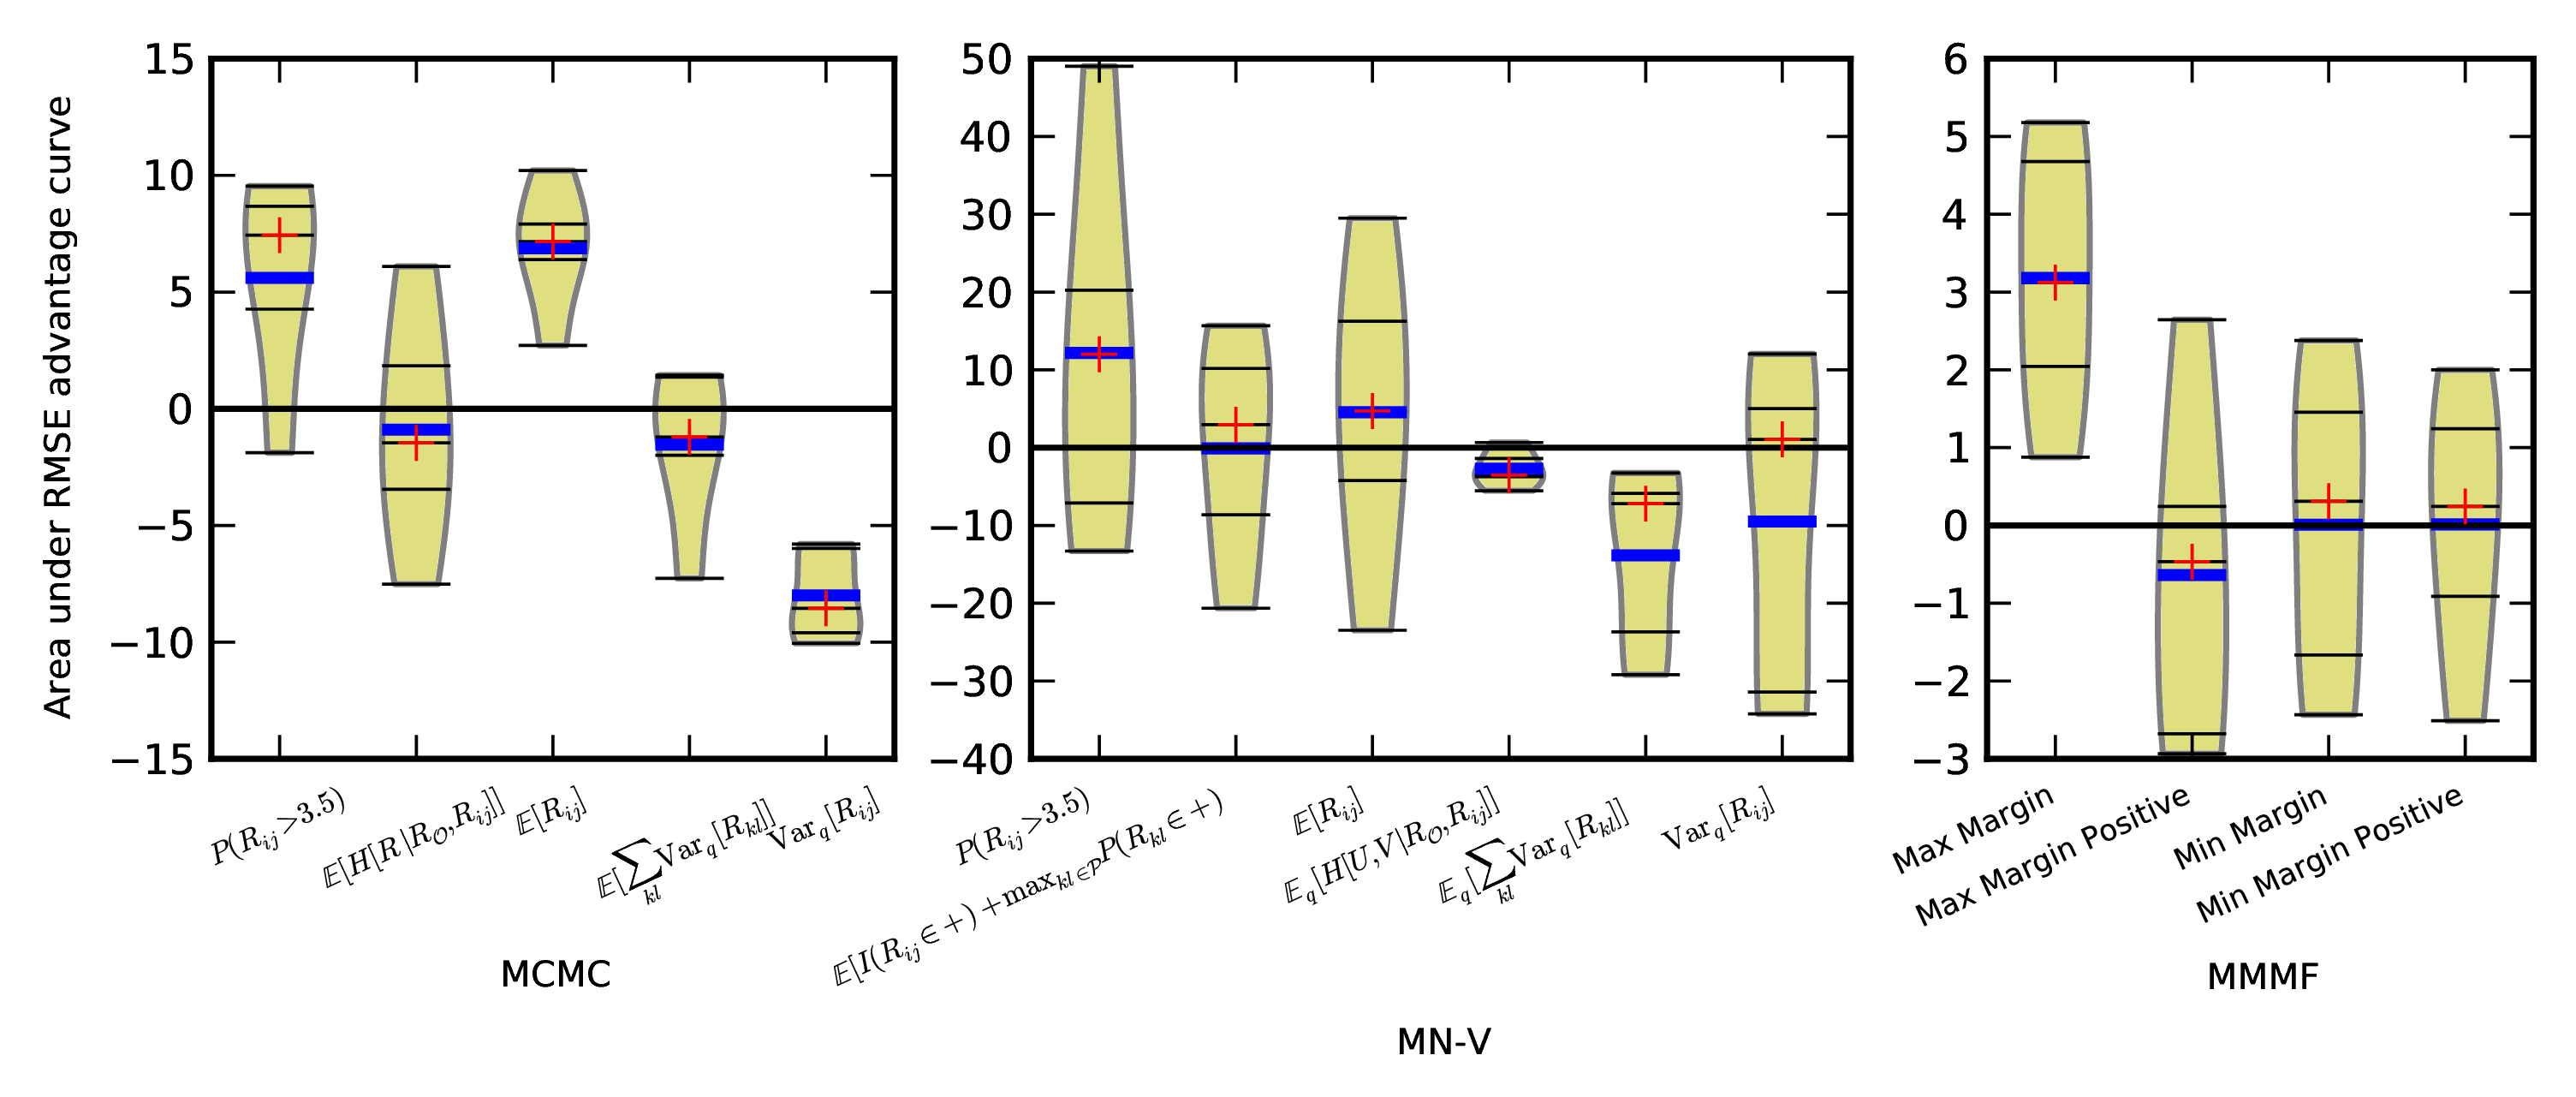
\includegraphics[width=\textwidth]{SutherlandPerformance}
    \else
      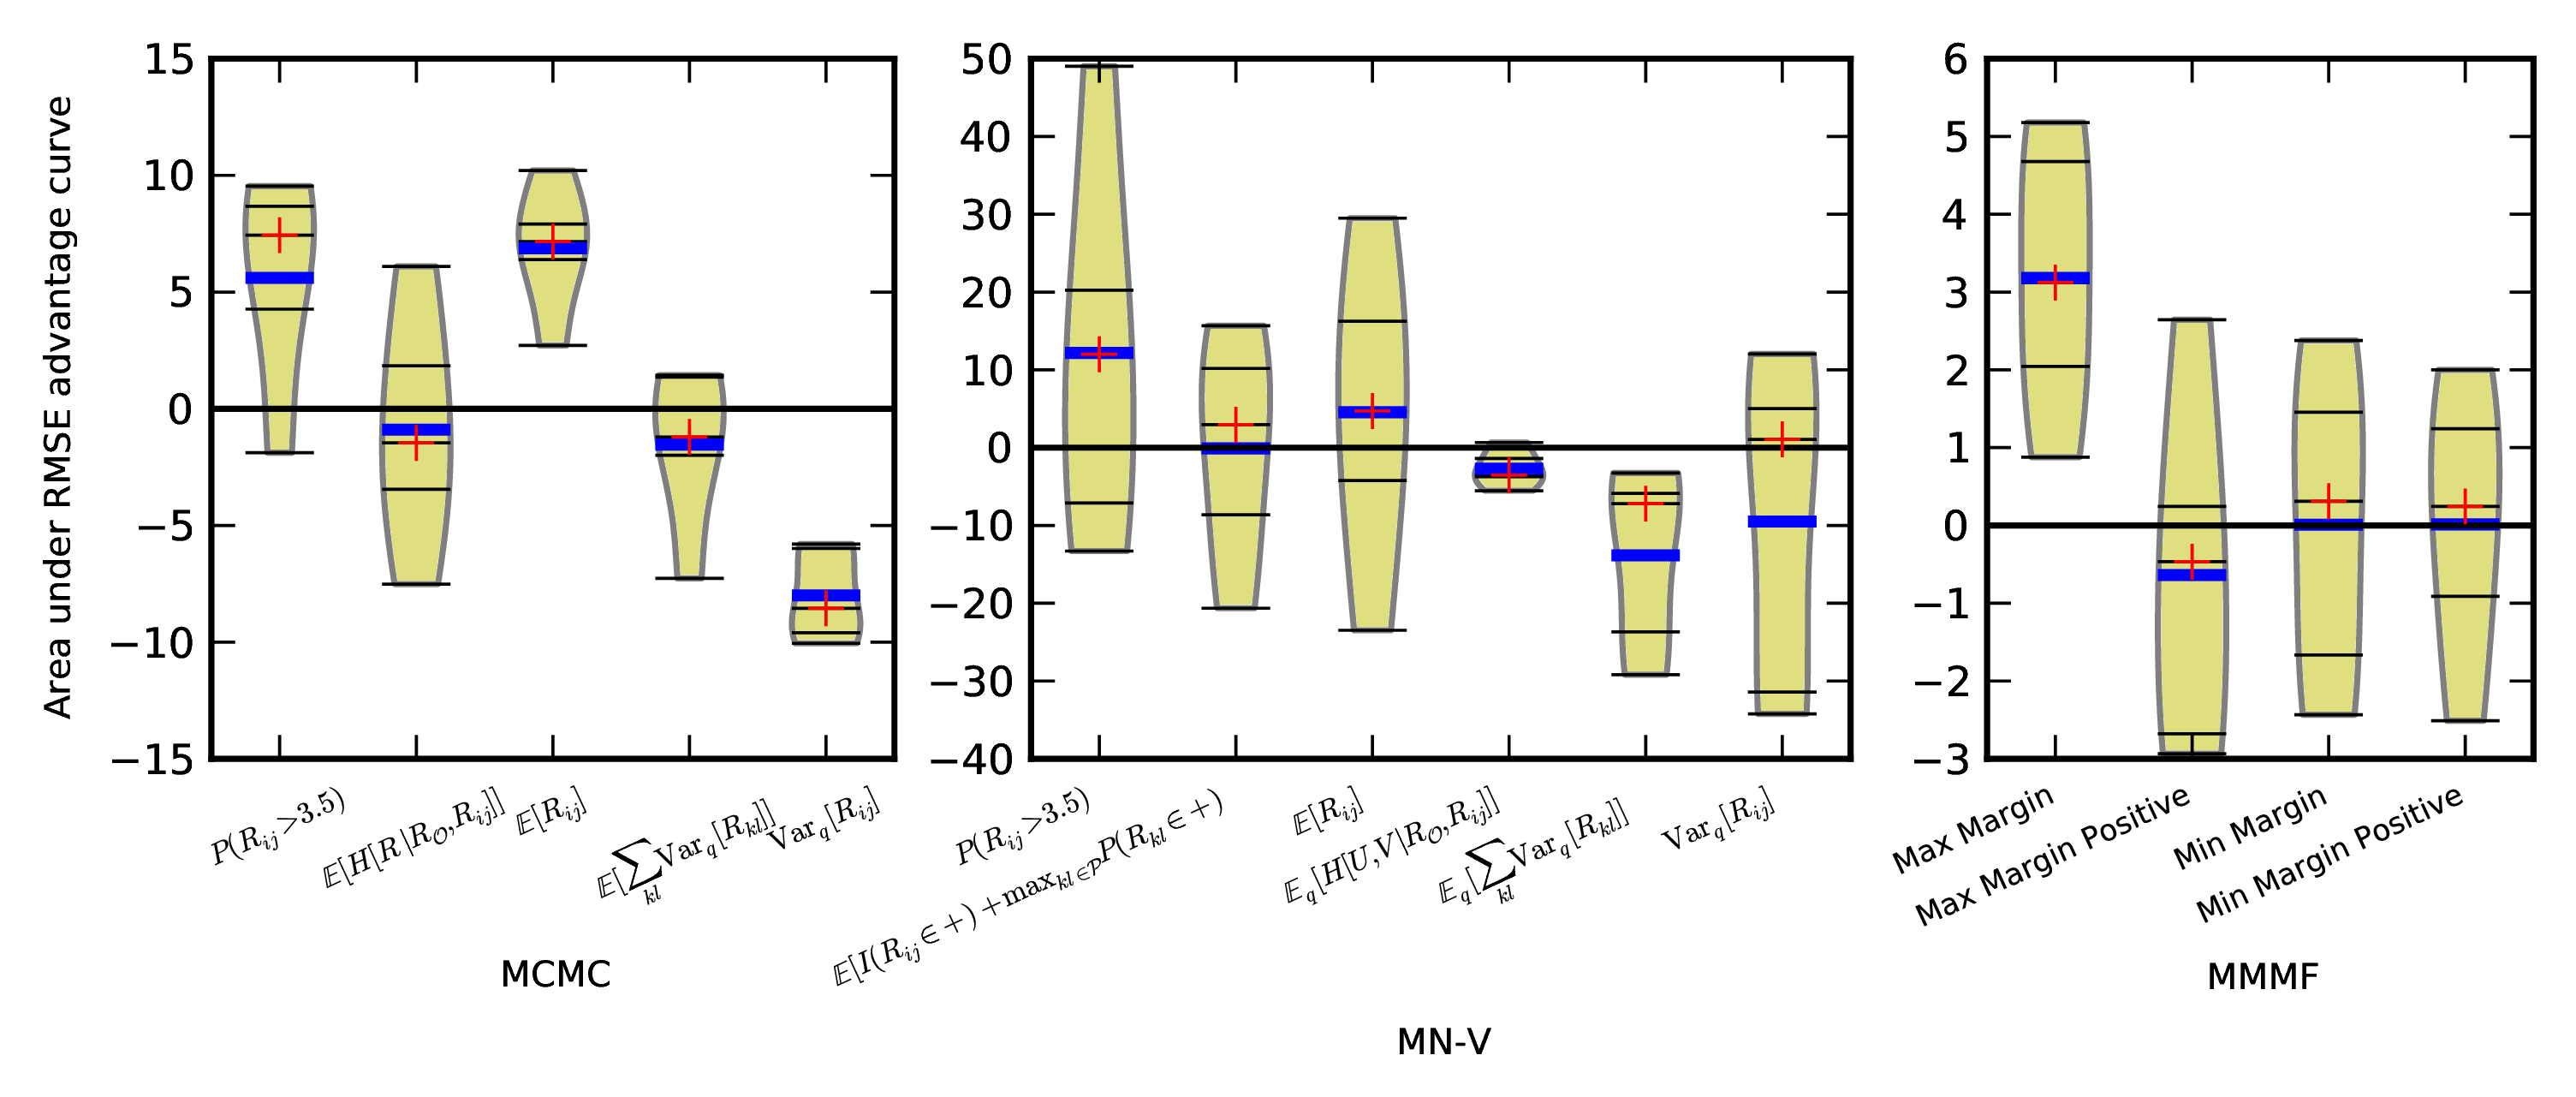
\includegraphics[bb = 92 86 545 742, width=\textwidth]{SutherlandPerformance}
    \fi
    \end{center}
This figure from Sutherland et al.'s paper \cite{active-mf} gives the prediction results of various techniques observed. The Area under RMSE advantage curve values represent the results of five runs of a $10 \times 10$ rank 1 continuous synthetic experiment against random sampling. Thus a negative value represents a method outperforming random selection.
  \begin{center}
    \leavevmode
    \ifpdf
      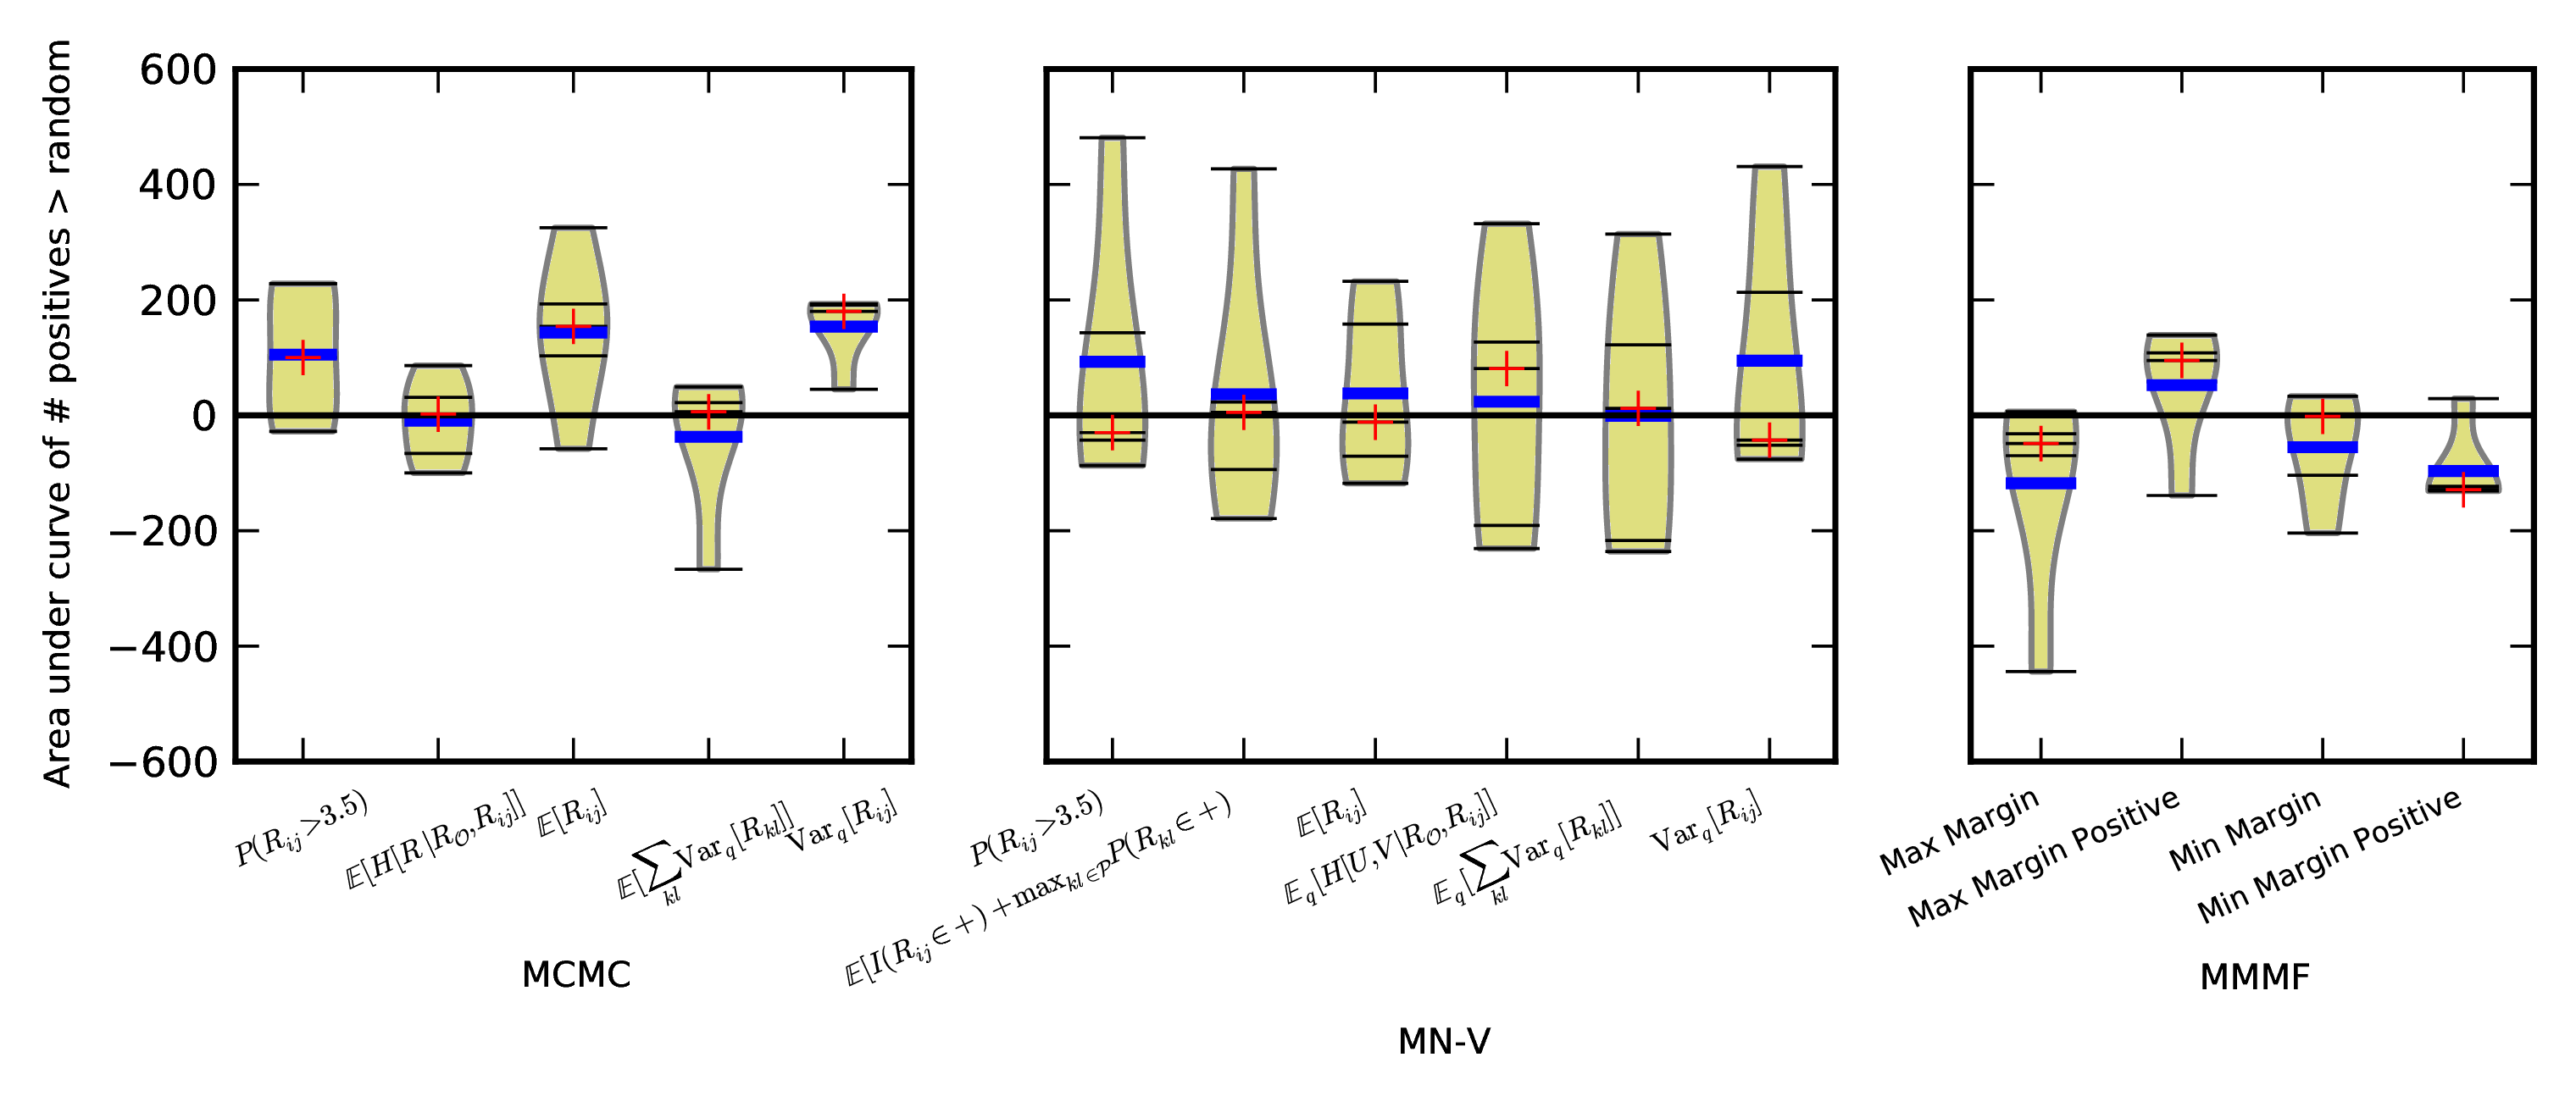
\includegraphics[width=\textwidth]{SutherlandPerformance_disc}
    \else
      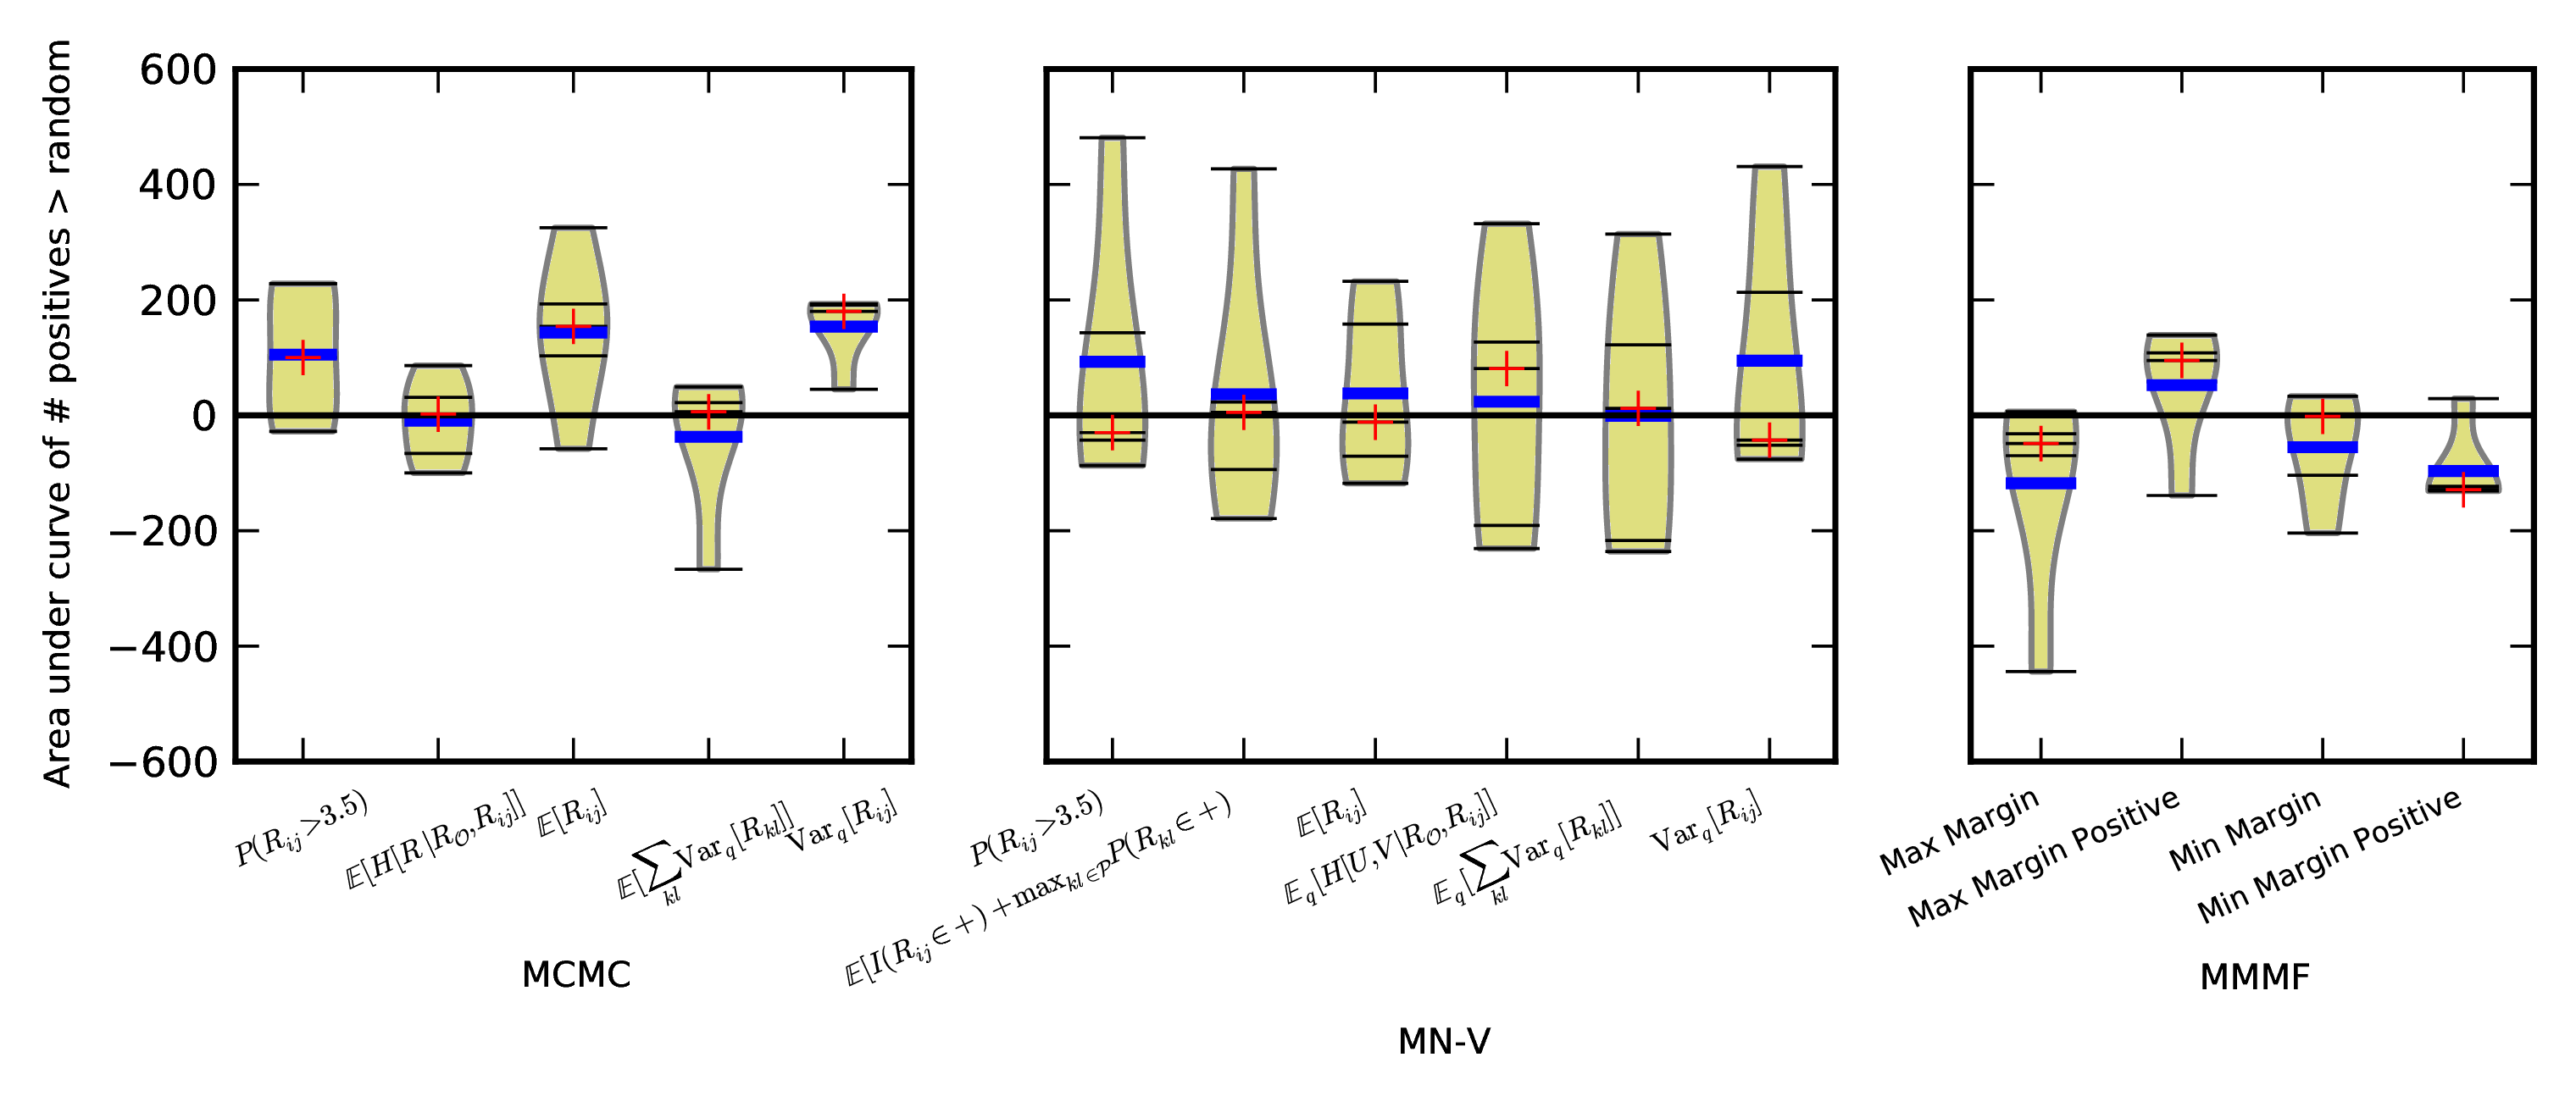
\includegraphics[bb = 92 86 545 742, width=\textwidth]{SutherlandPerformance_disc}
    \fi
    \end{center}
This figure gives the prediction results of various techniques observed for a synthetic discrete dataset. This time the measure is the number of useful values queried in a  $10 \times 10$ rank 4 discrete synthetic experiment against random sampling. A positive value represents a method outperforming random selection.

    \caption{Outline of the performance of algorithms proposed by Sutherland et al.}
    \label{fig:sutherland_alg}
\end{figure}
\nomenclature{MN-V}{Matrix-Normal Variational framework - Variational inference of the probability distribution of data in a matrix assuming Gaussian distribution}

\nomenclature{MMMF}{Maximum Margin Matrix Factorization - A collaborative prediction algorithm using low-norm instead of low-rank factorizations}

As can be seen, not all proposed methods performed well and even underperformed random selection. For this reason all Maximum Margin Matrix Factorization based methods are ignored, having little significant improvement over random selection. The two methods that exhibited good performance over the discrete and continuous datasets where the $\mathrm{Var}[R_{ij} \mid R_\mathcal{O}]$ searches, under Matrix-Normal and MCMC approximations. Thus, these will be the two algorithms implemented to be tested.

\section{Matrix-Normal Variance Search}
\label{sec:mnvar}
Here the idea is to infer the variance of unknown samples to be able to choose on to target. The variance is used as a proxy for uncertainty, where samples with a high variance are assumed to be the most "uncertain", due to being able to vary more.
\subsection{Derivation}
The value we seek for each sample is the variance of each individual sample given the observed set, that is $\mathrm{Var}[R_{ij} \mid R_\mathcal{O}]$. We derive it as such:
\begin{align*}
\mathrm{Var}[R_{ij} \mid R_\mathcal{O}] &= \mathbb{E} [\mathrm{Var}[R_{ij} \mid U,V] \mid R_\mathcal{O}] + \mathrm{Var} [\mathbb{E}[R_{ij} \mid U,V] \mid R_\mathcal{O}]\\
&= \mathbb{E}[\sigma^2] + \mathrm{Var}[\mathbf{u}_i^T \mathbf{v}_j \mid R_\mathcal{O}] \\
\mathrm{Var}[\mathbf{u}_i^T \mathbf{v}_j \mid R_\mathcal{O}] &= \mathrm{Var}\left[\sum\limits_{k=1}^{D} U_{ik}V_{jk} \mid R_\mathcal{O}\right] \\
&= \sum\limits_{k=1}^{D} \sum\limits_{l=1}^{D} \mathrm{Cov}[U_{ik}V_{jk},U_{il}V_{jl} \mid R_\mathcal{O}] \\
&= \sum\limits_{k=1}^{D} \sum\limits_{l=1}^{D} \mathbb{E}[U_{ik}V_{jk}U_{il}V_{jl} \mid R_\mathcal{O}] - \mathbb{E}[U_{ik}V_{jk} \mid R_\mathcal{O}] \mathbb{E}[U_{il}V_{jl} \mid R_\mathcal{O}]\\
\end{align*}


As $\mathbb{E}[\sigma^2]$ is a constant, we can ignore it. Now $\mathbb{E}[U_{ik}V_{jk} \mid R_\mathcal{O}]$ and $\mathbb{E}[U_{il}V_{jl} \mid R_\mathcal{O}]$ are not yet usable in their current form, we find their value via:
\begin{align*}
\mathbb{E}[X_a X_b] = \mathbb{E}[X_a] \mathbb{E}[X_b] + \mathrm{Cov}[X_a, X_b] = \mu_a\mu_b + \Sigma_{a,b}
\end{align*}
Where $\Sigma_{a,b}$ is the covariance matrix -  $\Sigma_{ab}= \mathrm{Cov}(X_a, X_b) = \mathbb{E}\left[
(X_a - \mu_a)(X_b - \mu_b)\right]$

The expression for $\mathbb{E}[U_{ik}V_{jk}U_{il}V_{jl} \mid R_\mathcal{O}]$ is slightly more complicated and requires the use of Isserlis' theorem \cite{isserlis1918}. Note that it assumes the random variables used are normal. 
\begin{align*}
\mathbb{E}[X_aX_bX_cX_d] &= \mu_a\mu_b\mu_c\mu_d +\mu_c\mu_d\Sigma{a,b}+\mu_b\mu_d\Sigma_{a,c}+\mu_b\mu_c\Sigma_{a,d}+\mu_a\mu_d\Sigma_{b,c}+\mu_a\mu_c\Sigma_{b,d}\\
&+\mu_a\mu_b\Sigma_{c,d} + \Sigma_{a,b}\Sigma_{c,d} + \Sigma_{a,c}\Sigma_{b,d} + \Sigma_{a,d}\Sigma_{b,c}
\end{align*}

To move from the $a,b,c,d$ coordinate system to $i,j,k,l$ to calculate $\mathrm{Var}[\mathbf{u}_i^T \mathbf{v}_j \mid R_\mathcal{O}]$ we create what is called the Matrix-Normal Framework approximation, which is a multivariate matrix assuming Gaussian distribution \cite{gupta1999matrix}.  For this we build a matrix system as such \cite{active-mf-slides}:
\begin{align}
\Sigma_{ij} = \mathrm{Cov}(\left[\begin{smallmatrix} U^T\\ V^T \end{smallmatrix}\right], \left[\begin{smallmatrix} U^T\\ V^T \end{smallmatrix}\right]) &=  
\begin{array}{c|c|c|c|c|c|c|c|c|}
  & \mathbf{u}_1 & \mathbf{u}_2 & \mathbf{u}_3 & \mathbf{u}_4 & \mathbf{u}_5 & \mathbf{v}_1 & \mathbf{v}_2 & \mathbf{v}_3 \\ \hline
\mathbf{u}_1  &  &   &   &   &   &  &  &  \\ \hline
\mathbf{u}_2 &  &   &   &   &   &  &  &  \\ \hline
\mathbf{u}_3  &  &   &   &   &   &  &  &  \\ \hline
\mathbf{u}_4  &  &   &   &   &   &  &  &  \\ \hline
\mathbf{u}_5  &  &   &   &   &   &  &  &  \\ \hline
\mathbf{v}_1  &  &   &   &   &   &  &  &  \\ \hline
\mathbf{v}_2  &  &   &   &   &   &  &  &  \\ \hline
\mathbf{v}_3  &  &   &   &   &   &  &  &  \\ \hline
\end{array} \label{eq:sigma_cov} \\
\Omega_{kl} =  \mathrm{Cov}(\left[\begin{smallmatrix} U & V \end{smallmatrix}\right], \left[\begin{smallmatrix} U & V \end{smallmatrix}\right]) &= 
\begin{array}{c|c|c|c|c|}
  & \mathbf{f}_1 & \mathbf{f}_2 & \mathbf{f}_3 & \mathbf{f}_4  \\ \hline
\mathbf{f}_1  &  &   &   &    \\ \hline
\mathbf{f}_2 &  &   &   &     \\ \hline
\mathbf{f}_3  &  &   &   &    \\ \hline
\mathbf{f}_4  &  &   &   &    \\ \hline
\end{array} \label{eq:omega_cov}
\end{align}

That is we assemble $U$ and $V$ into a single matrix and create the covariance matrices $\Sigma$ and $\Omega$. $\Sigma$ is the covariance of the features of each row ($U$) and column ($V$), thus $\Sigma \in \mathbb{R}^{(M+N)\times (M+N)}$. $\Omega$ is the covariance of the features themselves, thus $\Omega \in \mathbb{R}^{D\times D}$. This is used to get the full covariance matrix over all features of rows and columns by $\Sigma \otimes \Omega$.

From this we can consider $U$ and $V$ to be one variable, thus $\mathbb{E}[U_{ik}V_{jl}] = \mathbb{E}[X_{a}X_{b}]$ where $a = (i,j)$ and $b=(k,l)$. This gives:
\begin{align*}
\mathbb{E}[X_a X_b]  &= \mu_a\mu_b + \Sigma_{a,b}\\
&=\mathbb{E}[U_{ik}V_{jl}] = U_{ik}V_{jl} + \Sigma_{ij} \Omega_{kl}
\end{align*}
The indices $i,j$ refer to the $U,V$ coordinates in $\Sigma$ in equation \ref{eq:sigma_cov}. $k,l$ refers to the coordinates of the features of $\Omega$ in equation \ref{eq:omega_cov}. Note that the complexity to calculate $\Sigma$ and $\Omega$ combined is $O(D^3+(N+M)^3)$. Additionally note that $U_{ik}V_{jl}$ are used as means taken from the PMF best fit - while not ideal is an assumption required for calculation \cite{active-mf}.

\subsection{Performance}

This was first tested on the same $80\times 50$ synthetic data as in previous experiments and while the performance was good, it tended to "edge out" after more than 25\% of the dataset became available. A typical run is show in figure \ref{fig:MN-V-perf}. This is consistent with the performance reported by Sutherland et al. in figure \ref{fig:sutherland_alg}. 

  \begin{figure}[!htbp]
    \begin{center}
      \resizebox{\textwidth}{!}{% This file was created by matlab2tikz v0.4.7 running on MATLAB 8.1.
% Copyright (c) 2008--2014, Nico Schlömer <nico.schloemer@gmail.com>
% All rights reserved.
% Minimal pgfplots version: 1.3
% 
% The latest updates can be retrieved from
%   http://www.mathworks.com/matlabcentral/fileexchange/22022-matlab2tikz
% where you can also make suggestions and rate matlab2tikz.
% 
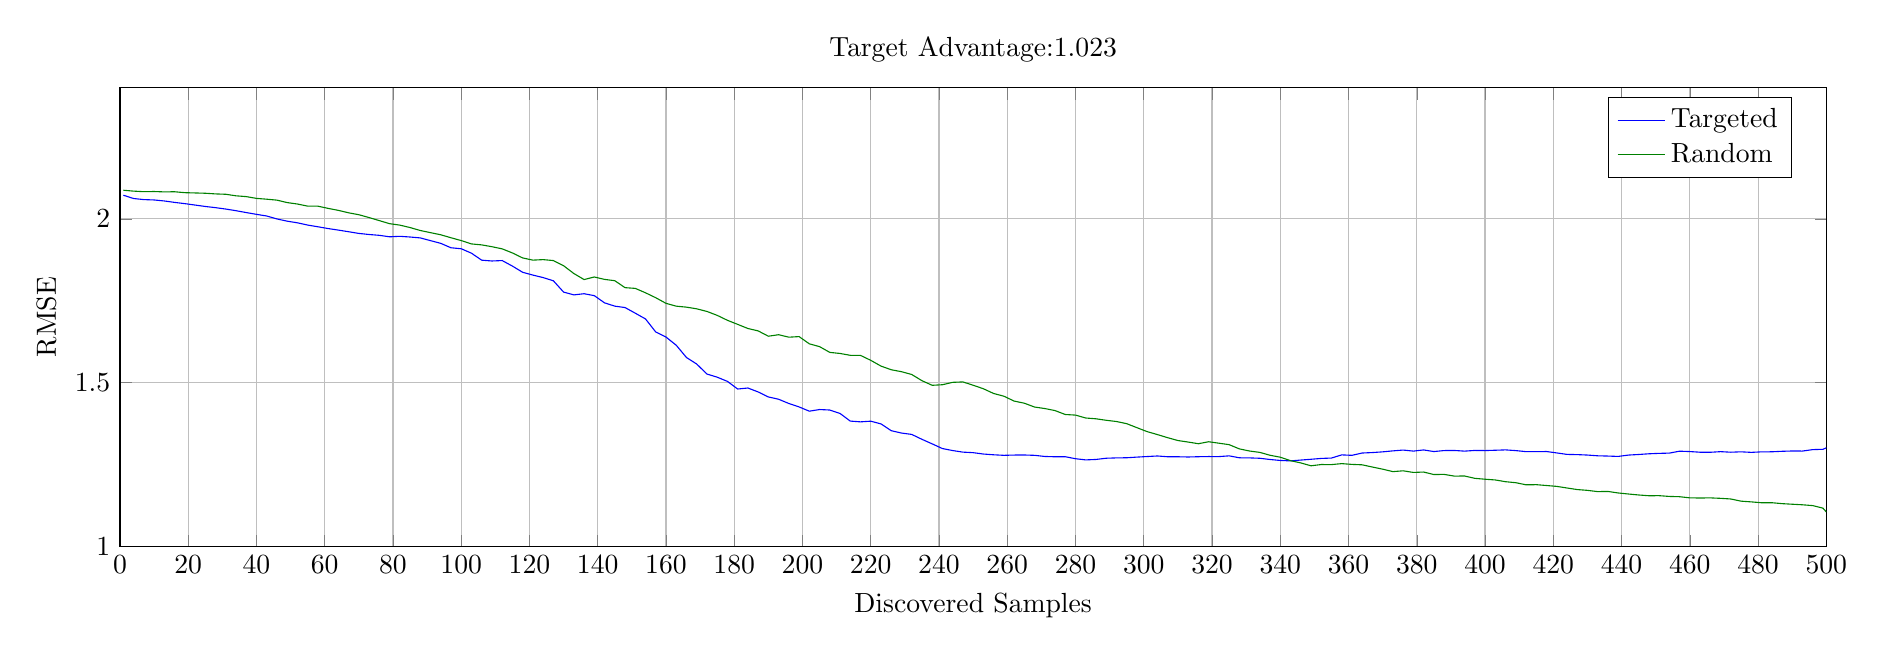
\begin{tikzpicture}

\begin{axis}[%
width=8.53186185641769in,
height=2.2921875in,
scale only axis,
xmin=0,
xmax=500,
xlabel={Discovered Samples},
xmajorgrids,
ymin=1,
ymax=2.4,
ylabel={RMSE},
ymajorgrids,
title={Target Advantage:1.023},
legend style={draw=black,fill=white,legend cell align=left}
]
\addplot [color=blue,solid]
  table[row sep=crcr]{1	2.07217796492918\\
4	2.06212270493792\\
7	2.05882437356678\\
10	2.05770772310212\\
13	2.05463256819977\\
16	2.05029038999817\\
19	2.04649955568304\\
22	2.04214711050768\\
25	2.03784797301423\\
28	2.03423279648376\\
31	2.02993729993713\\
34	2.02491635055087\\
37	2.01922342208279\\
40	2.01378732920106\\
43	2.00872741451322\\
46	1.99976064873121\\
49	1.99293235568156\\
52	1.98793139275403\\
55	1.98110244914886\\
58	1.97582861008334\\
61	1.97037647217666\\
64	1.96568743235825\\
67	1.96067642065653\\
70	1.95553225814245\\
73	1.95222363231337\\
76	1.94968837600179\\
79	1.94519452757987\\
82	1.94671582574677\\
85	1.94456924839872\\
88	1.94184800352677\\
91	1.93349583223219\\
94	1.92521848332823\\
97	1.91172130596277\\
100	1.90872882346895\\
103	1.8951253682236\\
106	1.87382958242028\\
109	1.87133938997235\\
112	1.87267011501452\\
115	1.85575306466301\\
118	1.83687065850172\\
121	1.82824122276525\\
124	1.82068993413038\\
127	1.81087884392425\\
130	1.77638745622223\\
133	1.76782438413003\\
136	1.77138943510964\\
139	1.76545820964674\\
142	1.74346779835438\\
145	1.73344175033161\\
148	1.72913726284919\\
151	1.71195929165539\\
154	1.69433936018818\\
157	1.65448344243473\\
160	1.63908694767779\\
163	1.61406681384958\\
166	1.57657630015616\\
169	1.5566917565721\\
172	1.52609994092278\\
175	1.51652904610699\\
178	1.50368856939048\\
181	1.48034402085276\\
184	1.4834528761387\\
187	1.47143288411547\\
190	1.45616474257825\\
193	1.44914891665654\\
196	1.43612670123312\\
199	1.4256581573023\\
202	1.41268358703128\\
205	1.41771340661325\\
208	1.41622550427769\\
211	1.40570120787203\\
214	1.38237721813787\\
217	1.38011853506596\\
220	1.3821246187814\\
223	1.37381796929417\\
226	1.35312809052608\\
229	1.34590495237109\\
232	1.34172684008272\\
235	1.32677225750146\\
238	1.3128521315865\\
241	1.2985509003513\\
244	1.29244945131536\\
247	1.28763987729826\\
250	1.28600061641922\\
253	1.28182325718132\\
256	1.27951413932043\\
259	1.27785169964859\\
262	1.27868774427141\\
265	1.27889345984466\\
268	1.27784137986272\\
271	1.27440947077995\\
274	1.27345121745604\\
277	1.2735928261685\\
280	1.26750193622842\\
283	1.26391104521067\\
286	1.26528659700911\\
289	1.26901035717902\\
292	1.27001218520397\\
295	1.27045536007768\\
298	1.27244298118008\\
301	1.2741919126503\\
304	1.27586897349281\\
307	1.27351270608901\\
310	1.27347313801709\\
313	1.27278813577858\\
316	1.27363043193357\\
319	1.27414402457253\\
322	1.27397896515088\\
325	1.27627622196343\\
328	1.27034812716924\\
331	1.27000627074729\\
334	1.2688956149271\\
337	1.26510646390248\\
340	1.26219130517703\\
343	1.2609059246488\\
346	1.26338860069923\\
349	1.26582053648389\\
352	1.26838961520604\\
355	1.26955477380922\\
358	1.27923001828898\\
361	1.27787091977098\\
364	1.28491935067654\\
367	1.28632801279594\\
370	1.2884657736677\\
373	1.29146883806027\\
376	1.29393893355191\\
379	1.29077127223434\\
382	1.29432065066798\\
385	1.28937288250242\\
388	1.29241691857647\\
391	1.2926933454363\\
394	1.29068756028848\\
397	1.29278769210034\\
400	1.29239303326408\\
403	1.29338884344584\\
406	1.2944748838647\\
409	1.29229343793145\\
412	1.28914655804349\\
415	1.28899567267332\\
418	1.28948087633663\\
421	1.28524664406664\\
424	1.28067337280748\\
427	1.28003038581361\\
430	1.2786961804855\\
433	1.27642714256949\\
436	1.27562242107382\\
439	1.27450140845304\\
442	1.27861911267101\\
445	1.28040813099069\\
448	1.28257635215677\\
451	1.28385629785686\\
454	1.28464215850466\\
457	1.29051195243648\\
460	1.28936667759647\\
463	1.28736885772353\\
466	1.28715448817792\\
469	1.28908509561051\\
472	1.28738485746969\\
475	1.28857929723097\\
478	1.2868948476176\\
481	1.28845828893595\\
484	1.2886646594279\\
487	1.29015662030612\\
490	1.29112064688728\\
493	1.29087869993448\\
496	1.29532409422768\\
499	1.29620725378601\\
500	1.30079161418323\\
};
\addlegendentry{Targeted};

\addplot [color=black!50!green,solid]
  table[row sep=crcr]{1	2.08737177550677\\
4	2.08467184403021\\
7	2.08298650087891\\
10	2.08348084945761\\
13	2.08235832565932\\
16	2.08278336567022\\
19	2.07997182596675\\
22	2.07911563225928\\
25	2.07822621974444\\
28	2.07619799809029\\
31	2.07509690461574\\
34	2.07037368540558\\
37	2.06796467565784\\
40	2.06249287777274\\
43	2.06005976089149\\
46	2.05720714465723\\
49	2.0496930022108\\
52	2.04530723149985\\
55	2.03888774106181\\
58	2.03873361093176\\
61	2.03199201729195\\
64	2.02591876819778\\
67	2.01848311414454\\
70	2.01262361605077\\
73	2.00395155190626\\
76	1.99462540594667\\
79	1.9852882756053\\
82	1.98091641778124\\
85	1.97347796749868\\
88	1.96446618648546\\
91	1.95785514086079\\
94	1.95138422004017\\
97	1.94229146720604\\
100	1.93366901648982\\
103	1.92342241018382\\
106	1.92051777604366\\
109	1.91496899516326\\
112	1.90839163752708\\
115	1.89586488086919\\
118	1.88066140255096\\
121	1.87395392292007\\
124	1.87550781674251\\
127	1.87264828173258\\
130	1.85683936289269\\
133	1.83307619089402\\
136	1.81464118524864\\
139	1.82249171408737\\
142	1.81510203517035\\
145	1.81115487870425\\
148	1.78991566680894\\
151	1.78768268232496\\
154	1.77419933459181\\
157	1.75914470656101\\
160	1.74201480568861\\
163	1.73337351081135\\
166	1.73037832871174\\
169	1.72524028710671\\
172	1.7172640519419\\
175	1.70530684126998\\
178	1.69022289382998\\
181	1.67781688837803\\
184	1.6651866018857\\
187	1.65786833325152\\
190	1.64163461056598\\
193	1.64621427296132\\
196	1.6386410457844\\
199	1.64045407738492\\
202	1.61837347420205\\
205	1.60981307131975\\
208	1.59221952958318\\
211	1.58892920883708\\
214	1.58329322993786\\
217	1.58301614026078\\
220	1.567965103681\\
223	1.55038370751194\\
226	1.53919574761702\\
229	1.53327736766467\\
232	1.52476495571093\\
235	1.50581086034833\\
238	1.49171998420279\\
241	1.49342951724959\\
244	1.5007717380585\\
247	1.50204426605883\\
250	1.49192696470451\\
253	1.48121566474336\\
256	1.46672052014451\\
259	1.45844805265428\\
262	1.44355779059618\\
265	1.43703738035327\\
268	1.4253302052287\\
271	1.42074401790011\\
274	1.41449212897748\\
277	1.40253724549153\\
280	1.40069222665835\\
283	1.39180532175089\\
286	1.38940725648008\\
289	1.38487970543042\\
292	1.38110597813458\\
295	1.3745230010058\\
298	1.36230351141792\\
301	1.3501871378517\\
304	1.3412095644929\\
307	1.33173351861769\\
310	1.32304550636488\\
313	1.31840292381511\\
316	1.31334104190201\\
319	1.31933152266431\\
322	1.31495091989763\\
325	1.31047964925082\\
328	1.29756420173432\\
331	1.29097480308478\\
334	1.28685145817632\\
337	1.27805122623317\\
340	1.27212012515377\\
343	1.26156765537743\\
346	1.2546533090913\\
349	1.2459105816125\\
352	1.24972460480505\\
355	1.24957136202949\\
358	1.25251678013392\\
361	1.25017249793226\\
364	1.24889540351554\\
367	1.24207233711686\\
370	1.23558814397032\\
373	1.22809686061264\\
376	1.23060254216309\\
379	1.22558605980194\\
382	1.22682227549603\\
385	1.21920191679697\\
388	1.21968643397675\\
391	1.21442053358153\\
394	1.21472677378805\\
397	1.2076025372052\\
400	1.20488826736279\\
403	1.20264160565174\\
406	1.19732675748935\\
409	1.19427745019973\\
412	1.18787560986912\\
415	1.18824687142166\\
418	1.18569285163679\\
421	1.18301310411735\\
424	1.17815756614337\\
427	1.1733234895432\\
430	1.170920066358\\
433	1.16705564895868\\
436	1.16758311592514\\
439	1.16291304863818\\
442	1.15974434515618\\
445	1.15677495393665\\
448	1.15445458443966\\
451	1.15467135208282\\
454	1.15233728237269\\
457	1.15149389611694\\
460	1.1479855493612\\
463	1.14753512073225\\
466	1.14791346977819\\
469	1.14654344230593\\
472	1.14456063957849\\
475	1.13791032233366\\
478	1.13570570496753\\
481	1.13306893975319\\
484	1.13318773014601\\
487	1.13032176593801\\
490	1.12855069123371\\
493	1.12682279115302\\
496	1.12434455628116\\
499	1.11658124448945\\
500	1.10494857330348\\
};
\addlegendentry{Random};

\end{axis}
\end{tikzpicture}%}
    \end{center}
    Performed on Synthetic Data.
      \caption{Matrix Normal Maximum Variance Search}
      \label{fig:MN-V-perf}
  \end{figure}
  
  
\subsubsection{Improving Performance}

Calculating the variance has a complexity of about $O(MND^2)$ in addition to the calculation of the covariance matrices, thus calculating the criteria at each new sample is not ideal. These tweaks were done to improve performance: 

\begin{description}[style=standard,leftmargin=.7cm,font=\bfseries]
  \item[Variance Matrix Calculation Update] Rather than calculating the matrix everytime a new sample comes in, we calculate the matrix at fixed intervals of incoming samples, for example after 10 have been requested.
  \item[Memory Optimisation] There are many combinations of $\mathbb{E}[U_{ik}V_{jl}]$ over the double summation. To optimise, we use the symmetry property of the covariance matrix and locally cache already calculated values.
  \item[Unknown Samples] We only calculate the variance for unknown samples.
  \item[Online Updating] When $U$ and $V$ are calculated online it is also possible to gradually update the variance matrix.

\end{description}

Basic memory optimisation alone allowed the execution to be more than halved. In the case of a $80 \times 50$ matrix with $D=7$, from 1.81 seconds down to 0.81 seconds on average.


\section{MCMC Variance Search}
\label{sec:mcmcvar}
From results obtained in simulations as well as Sutherland et al.'s we saw that the Matrix-Normal Variance Search performed reasonably well, but had instances of under performing random selection. One of the reasons for this was that the data distribution was not entirely reflected in $U$ and $V$ used to calculate $\mathrm{Var}[\mathbf{u}_i^T \mathbf{v}_j \mid R_\mathcal{O}]$. 
\subsection{Derivation}
Here we keep the same equations for $\mathrm{Var}[\mathbf{u}_i^T \mathbf{v}_j \mid R_\mathcal{O}]$ but instead take $U$ and $V$ from an estimate sampled across the expected distribution of data. In BPMF, section \ref{sec:bpmf}, we had $U$ and $V$ expressed as:

\begin{align*}
P(U,V|R,\Theta_U,\Theta_V) =\int \int P(R | U,V) P(U,V | R,\Theta_U,\Theta_V) P(\Theta_U,\Theta_V | \Theta_0)d\Theta_U d\Theta_V
\end{align*}

Unfortunately an analytical solution is difficult to achieve and we instead rely on approximation methods. For quick intuition on how this works consider the following, simplified, function \cite{mcmc-int}:
\begin{align*}
I = \int g(\theta)p(\theta)d\theta
\end{align*}
Where $g(\theta)$ is a function of $\theta$ and $p(\theta)$ is the distribution of this variable. In cases where this is not possible we resort to Monte-Carlo Markov Chain Integration:
\begin{align*}
\hat{I}_M =\frac{1}{M} \sum\limits_{i=1}^{M} g(\theta ^{(i)}) 
\end{align*}

Where $M$ is the number of values sampled and $i$ the index. We have that as $M \to \infty$, $\hat{I}_M = I$. By process of iteration and random sampling the real distribution is approached and $\hat{I}_M$ is used instead of $I$.This is the process we will use to sample from the already known values.


 Sutherland et al.\cite{active-mf} use Hamiltonian Monte Carlo sampling methods but here we will use Gibbs Sampling, in a similar way to Salakhutdinov and Mnih \cite{SalMnih2008} in BPMF. Algorithm \ref{alg:gibbs_pmf} describes the process to sample from $V$, which is exactly the same for $U$. A $U$ and $V$ obtained via PMF are used as inputs.


\begin{algorithm}
\caption{Gibbs Sampling for BPMF}\label{alg:gibbs_pmf}
\begin{algorithmic}[1]
\Procedure{GibbsSamplingForV}{$U$,$V$,$R$}
\For{j=1..M} 
\State{$row_{in} = $row indices of known samples in column $j$} 
\State{$\mathcal{M} = U_{index = row_{in}}$} \Comment{Get feature vectors of known rows in column $j$}
\State{$\mathbf{r} = R_{row_{in},j}$} \Comment{Vector of known values in column $j$}
\State{$C = (\alpha_V+\beta\cdot\mathcal{M}^T\mathcal{M})^{-1}$} \Comment{Covariance of known feature vectors $U$}
\State{$\mu_V = C\cdot(\beta\cdot\mathcal{M}^T\mathbf{r}+\alpha_V \mu_V)$} \Comment{Update mean vector}
\State{$\Lambda = \text{Cholesky}(C)$} \Comment{Cholesky upper triangular decomposition}
\State{$\mathbf{x} \sim \mathcal{N}(0,1) \in \mathbf{R}^D$} \Comment{Randomly sample $D$ variables from Normal}
\State{$V_{j}=\Lambda\mathbf{x}+\mu_V$} \Comment{Update $V$}
\EndFor
\State \textbf{return} $V$
\EndProcedure
\end{algorithmic}
\end{algorithm}


$\alpha_V$ is the precision hyperparameter for $V$ and it is used to ensure non-singularity of $C$. $\mu_V$ is the average vector. $\beta$ is a parameter used for the Inverse-Wishart distribution, used as the prior of covariance matrix from data assumed to be from a normal distribution. Details are available in the appendix \ref{sec:app_bpmf}. We take $\Lambda$ as the Cholesky decomposition of the covariance $C$. If applied to a vector of uncorrelated samples ($\mathbf{x}$) it produces a vector with covariances of sampled system, which is why we add it to $\mu_V$, creating a feature vector of the samples.  Note that hyperparameters are reinitialised each loop before sampling trials.


In simpler terms, we capture the properties of the current distribution of known values in $V_j$ in $C$ and using the Cholesky decomposition update V with samples randomly generated from the captured distribution. Repeating this a few times(for our case, 3) over $U$ and $V$ asymptotically captures the real distribution of the samples. 

From this we get a better estimate of $\mathrm{Var}[\mathbf{u}_i^T \mathbf{v}_j \mid R_\mathcal{O}]$ and select the highest value for sampling.
\subsection{Performance}

MCMC Maximum Variance search was done on figure \ref{fig:MN-V-varsearch} and \ref{fig:eiffel_max_var_search}. As we see the performance on the synthetic data was better than the Matrix Normal version, being able to always perform better than random sampling. It should be noted that for image discovery, as in \ref{fig:eiffel_max_var_search}, MCMC performed less well than the clustered search (compare to figure \ref{fig:eiffel_clustering_random}) - this was observed over multiple runs. Finally the running speed was found to be quite a lot slower, taking 0.8 seconds on average compared to 0.01 for clustered knowledge search to calculate the criteria for sample selection.

 \begin{figure}[!htbp]
   \begin{center}
     \resizebox{\textwidth}{!}{% This file was created by matlab2tikz v0.4.7 running on MATLAB 8.1.
% Copyright (c) 2008--2014, Nico Schlömer <nico.schloemer@gmail.com>
% All rights reserved.
% Minimal pgfplots version: 1.3
% 
% The latest updates can be retrieved from
%   http://www.mathworks.com/matlabcentral/fileexchange/22022-matlab2tikz
% where you can also make suggestions and rate matlab2tikz.
% 
\begin{tikzpicture}

\begin{axis}[%
width=2.19625603864734in,
height=2.2728125in,
scale only axis,
xmin=0,
xmax=500,
xlabel={Discovered Samples},
xmajorgrids,
ymin=1,
ymax=2.4,
ylabel={RMSE},
ymajorgrids,
name=plot2,
title={Target Advantage:1.101}
]
\addplot [color=blue,solid,forget plot]
  table[row sep=crcr]{1	2.06951517257059\\
4	2.0869975872509\\
7	2.08103952147042\\
10	2.0753586370514\\
13	2.07373094997347\\
16	2.07115788724271\\
19	2.06963278760257\\
22	2.06484829701644\\
25	2.05728474072855\\
28	2.05841876874843\\
31	2.05142040393897\\
34	2.04438283782421\\
37	2.0358378827621\\
40	2.03712717447943\\
43	2.03731928304517\\
46	2.04154246089513\\
49	2.0350907696424\\
52	2.03828846856109\\
55	2.04488617363075\\
58	2.03879522020787\\
61	2.03363206341838\\
64	2.00987760912885\\
67	1.99602788609993\\
70	1.97164138282284\\
73	1.95054864630478\\
76	1.92469610058144\\
79	1.91853158115475\\
82	1.90193328286329\\
85	1.90425862662948\\
88	1.91152026099947\\
91	1.91217207143605\\
94	1.89405756567734\\
97	1.88021435737431\\
100	1.86702306784919\\
103	1.84463901382843\\
106	1.81318359279943\\
109	1.77777954157781\\
112	1.74438394947764\\
115	1.73044030606485\\
118	1.68282482446093\\
121	1.68032799007376\\
124	1.64103715043388\\
127	1.62711314432135\\
130	1.60059786692634\\
133	1.6086073738429\\
136	1.60612772446024\\
139	1.57532684746015\\
142	1.57555558858191\\
145	1.60443069661882\\
148	1.6107264530929\\
151	1.59633161832539\\
154	1.59486975503252\\
157	1.60186704616335\\
160	1.59132800396157\\
163	1.57979444828184\\
166	1.55327712016505\\
169	1.52695020217204\\
172	1.48503561723383\\
175	1.46361196222446\\
178	1.42633534386435\\
181	1.3815195130784\\
184	1.35763139007661\\
187	1.3433293607386\\
190	1.34505611035272\\
193	1.34927391157997\\
196	1.33406699947773\\
199	1.34399067458741\\
202	1.34685210142679\\
205	1.34451743747387\\
208	1.33006709754534\\
211	1.31551394501568\\
214	1.31408054120038\\
217	1.29917342848288\\
220	1.2838708773734\\
223	1.28473716486946\\
226	1.27931207133722\\
229	1.27470806417715\\
232	1.27130976104606\\
235	1.2681680675065\\
238	1.27643001273846\\
241	1.27056735500564\\
244	1.27003699360378\\
247	1.26237545338544\\
250	1.25315174140016\\
253	1.24710990204099\\
256	1.24399576780197\\
259	1.24812043993773\\
262	1.23918620912122\\
265	1.23423616291519\\
268	1.23275946089628\\
271	1.22870511240745\\
274	1.2155502006172\\
277	1.20493507890713\\
280	1.19900001452417\\
283	1.19862449983493\\
286	1.18861520719581\\
289	1.18613325602982\\
292	1.17748914250914\\
295	1.1766082818931\\
298	1.17125805548398\\
301	1.16780129197513\\
304	1.16252174223498\\
307	1.15412543788157\\
310	1.15744194938611\\
313	1.15465722742835\\
316	1.15199780773044\\
319	1.14988120217212\\
322	1.15501969500764\\
325	1.15279631966572\\
328	1.15222520067874\\
331	1.15278100375271\\
334	1.15111366337206\\
337	1.15054899928969\\
340	1.15055951926519\\
343	1.14765576598283\\
346	1.14827532713664\\
349	1.14737785311683\\
352	1.14469310426331\\
355	1.14273598628017\\
358	1.13595567057849\\
361	1.13146339714016\\
364	1.12472785963559\\
367	1.12093205216107\\
370	1.11133516810054\\
373	1.10511844972657\\
376	1.09877137762578\\
379	1.0949949051823\\
382	1.09044378217313\\
385	1.088155156071\\
388	1.08277895896492\\
391	1.07935590780405\\
394	1.0761709990846\\
397	1.07464125838609\\
400	1.07208467178701\\
403	1.06940583850326\\
406	1.06768210001444\\
409	1.06926456105682\\
412	1.06888703911823\\
415	1.06721746615859\\
418	1.06842284405011\\
421	1.06936214467617\\
424	1.06885906707902\\
427	1.06657553825248\\
430	1.06821893090067\\
433	1.06526470180524\\
436	1.06290146189374\\
439	1.05973423310235\\
442	1.05521241228798\\
445	1.05466523364914\\
448	1.05429086184452\\
451	1.05287210332248\\
454	1.0535505854728\\
457	1.05368572421694\\
460	1.0567477941951\\
463	1.05485056230343\\
466	1.05670081813142\\
469	1.05486314573757\\
472	1.05383974165637\\
475	1.05321886705928\\
478	1.05402007791782\\
481	1.05743019581946\\
484	1.05833043980336\\
487	1.057233949908\\
490	1.05713232472705\\
493	1.06128921343148\\
496	1.05715155454772\\
499	1.05655653727356\\
500	1.05663171835569\\
};
\addplot [color=black!50!green,solid,forget plot]
  table[row sep=crcr]{1	2.08737177550677\\
4	2.08467184403021\\
7	2.08298650087891\\
10	2.08348084945761\\
13	2.08235832565932\\
16	2.08278336567022\\
19	2.07997182596675\\
22	2.07911563225928\\
25	2.07822621974444\\
28	2.07619799809029\\
31	2.07509690461574\\
34	2.07037368540558\\
37	2.06796467565784\\
40	2.06249287777274\\
43	2.06005976089149\\
46	2.05720714465723\\
49	2.0496930022108\\
52	2.04530723149985\\
55	2.03888774106181\\
58	2.03873361093176\\
61	2.03199201729195\\
64	2.02591876819778\\
67	2.01848311414454\\
70	2.01262361605077\\
73	2.00395155190626\\
76	1.99462540594667\\
79	1.9852882756053\\
82	1.98091641778124\\
85	1.97347796749868\\
88	1.96446618648546\\
91	1.95785514086079\\
94	1.95138422004017\\
97	1.94229146720604\\
100	1.93366901648982\\
103	1.92342241018382\\
106	1.92051777604366\\
109	1.91496899516326\\
112	1.90839163752708\\
115	1.89586488086919\\
118	1.88066140255096\\
121	1.87395392292007\\
124	1.87550781674251\\
127	1.87264828173258\\
130	1.85683936289269\\
133	1.83307619089402\\
136	1.81464118524864\\
139	1.82249171408737\\
142	1.81510203517035\\
145	1.81115487870425\\
148	1.78991566680894\\
151	1.78768268232496\\
154	1.77419933459181\\
157	1.75914470656101\\
160	1.74201480568861\\
163	1.73337351081135\\
166	1.73037832871174\\
169	1.72524028710671\\
172	1.7172640519419\\
175	1.70530684126998\\
178	1.69022289382998\\
181	1.67781688837803\\
184	1.6651866018857\\
187	1.65786833325152\\
190	1.64163461056598\\
193	1.64621427296132\\
196	1.6386410457844\\
199	1.64045407738492\\
202	1.61837347420205\\
205	1.60981307131975\\
208	1.59221952958318\\
211	1.58892920883708\\
214	1.58329322993786\\
217	1.58301614026078\\
220	1.567965103681\\
223	1.55038370751194\\
226	1.53919574761702\\
229	1.53327736766467\\
232	1.52476495571093\\
235	1.50581086034833\\
238	1.49171998420279\\
241	1.49342951724959\\
244	1.5007717380585\\
247	1.50204426605883\\
250	1.49192696470451\\
253	1.48121566474336\\
256	1.46672052014451\\
259	1.45844805265428\\
262	1.44355779059618\\
265	1.43703738035327\\
268	1.4253302052287\\
271	1.42074401790011\\
274	1.41449212897748\\
277	1.40253724549153\\
280	1.40069222665835\\
283	1.39180532175089\\
286	1.38940725648008\\
289	1.38487970543042\\
292	1.38110597813458\\
295	1.3745230010058\\
298	1.36230351141792\\
301	1.3501871378517\\
304	1.3412095644929\\
307	1.33173351861769\\
310	1.32304550636488\\
313	1.31840292381511\\
316	1.31334104190201\\
319	1.31933152266431\\
322	1.31495091989763\\
325	1.31047964925082\\
328	1.29756420173432\\
331	1.29097480308478\\
334	1.28685145817632\\
337	1.27805122623317\\
340	1.27212012515377\\
343	1.26156765537743\\
346	1.2546533090913\\
349	1.2459105816125\\
352	1.24972460480505\\
355	1.24957136202949\\
358	1.25251678013392\\
361	1.25017249793226\\
364	1.24889540351554\\
367	1.24207233711686\\
370	1.23558814397032\\
373	1.22809686061264\\
376	1.23060254216309\\
379	1.22558605980194\\
382	1.22682227549603\\
385	1.21920191679697\\
388	1.21968643397675\\
391	1.21442053358153\\
394	1.21472677378805\\
397	1.2076025372052\\
400	1.20488826736279\\
403	1.20264160565174\\
406	1.19732675748935\\
409	1.19427745019973\\
412	1.18787560986912\\
415	1.18824687142166\\
418	1.18569285163679\\
421	1.18301310411735\\
424	1.17815756614337\\
427	1.1733234895432\\
430	1.170920066358\\
433	1.16705564895868\\
436	1.16758311592514\\
439	1.16291304863818\\
442	1.15974434515618\\
445	1.15677495393665\\
448	1.15445458443966\\
451	1.15467135208282\\
454	1.15233728237269\\
457	1.15149389611694\\
460	1.1479855493612\\
463	1.14753512073225\\
466	1.14791346977819\\
469	1.14654344230593\\
472	1.14456063957849\\
475	1.13791032233366\\
478	1.13570570496753\\
481	1.13306893975319\\
484	1.13318773014601\\
487	1.13032176593801\\
490	1.12855069123371\\
493	1.12682279115302\\
496	1.12434455628116\\
499	1.11658124448945\\
500	1.10494857330348\\
};
\end{axis}

\begin{axis}[%
width=2.19625603864734in,
height=2.2728125in,
axis on top,
scale only axis,
xmin=0.5,
xmax=50.5,
y dir=reverse,
ymin=0.5,
ymax=80.5,
at=(plot2.left of south west),
anchor=right of south east,
title={Targeted RMSE:1.057}
]
\addplot [forget plot] graphics [xmin=0.5,xmax=50.5,ymin=0.5,ymax=80.5] {MN-V-varsearch-1.png};
\end{axis}

\begin{axis}[%
width=2.19625603864734in,
height=2.2728125in,
axis on top,
scale only axis,
xmin=0.5,
xmax=50.5,
y dir=reverse,
ymin=0.5,
ymax=80.5,
at=(plot2.right of south east),
anchor=left of south west,
title={Targeted Samples}
]
\addplot [forget plot] graphics [xmin=0.5,xmax=50.5,ymin=0.5,ymax=80.5] {MN-V-varsearch-2.png};
\end{axis}
\end{tikzpicture}%}
   \end{center}
   PMF with $\lambda = 0.01$ and an initial 1.25\% of samples discovered
     \caption{MCMC Maximum Variance Search}
     \label{fig:MN-V-varsearch}
 \end{figure}
 
\begin{figure}[!htbp]
  \begin{center}
    \resizebox{\textwidth}{!}{% This file was created by matlab2tikz v0.4.7 running on MATLAB 8.1.
% Copyright (c) 2008--2014, Nico Schlömer <nico.schloemer@gmail.com>
% All rights reserved.
% Minimal pgfplots version: 1.3
% 
% The latest updates can be retrieved from
%   http://www.mathworks.com/matlabcentral/fileexchange/22022-matlab2tikz
% where you can also make suggestions and rate matlab2tikz.
% 
\begin{tikzpicture}

\begin{axis}[%
width=2.25in,
height=2.5in,
axis on top,
scale only axis,
xmin=0.5,
xmax=50.5,
y dir=reverse,
ymin=0.5,
ymax=80.5,
name=plot2,
title={Targeted RMSE:0.821}
]
\addplot [forget plot] graphics [xmin=0.5,xmax=50.5,ymin=0.5,ymax=80.5] {eiffel_max_var_search-1.png};
\end{axis}

\begin{axis}[%
width=2.25in,
height=2.5in,
axis on top,
scale only axis,
xmin=0.5,
xmax=50.5,
y dir=reverse,
ymin=0.5,
ymax=80.5,
at=(plot2.left of south west),
anchor=right of south east,
title={Random RMSE:0.817}
]
\addplot [forget plot] graphics [xmin=0.5,xmax=50.5,ymin=0.5,ymax=80.5] {eiffel_max_var_search-2.png};
\end{axis}

\begin{axis}[%
width=2.25in,
height=2.5in,
scale only axis,
xmin=0,
xmax=1000,
xlabel={Discovered Samples},
xmajorgrids,
ymin=0.5,
ymax=3.5,
ylabel={RMSE},
ymajorgrids,
name=plot3,
at=(plot2.right of south east),
anchor=left of south west,
title={Target Advantage:1.027}
]
\addplot [color=blue,solid,forget plot]
  table[row sep=crcr]{1	3.23096646698746\\
4	3.24289052919744\\
7	3.2390809556552\\
10	3.23784580658611\\
13	3.23535124900901\\
16	3.23246063948494\\
19	3.23359170526017\\
22	3.23138581919351\\
25	3.22837860844063\\
28	3.22798392715434\\
31	3.22476271541435\\
34	3.22366304028217\\
37	3.21700505308898\\
40	3.21042504654905\\
43	3.20527761098874\\
46	3.19051228337716\\
49	3.18258795316644\\
52	3.17679682746987\\
55	3.17774282636235\\
58	3.15982500229946\\
61	3.15813379408625\\
64	3.14056835581721\\
67	3.12228092457842\\
70	3.09401164331764\\
73	3.07785293458209\\
76	3.05480096556554\\
79	3.05244552498845\\
82	3.03197249361327\\
85	3.0218687588786\\
88	3.01235632035684\\
91	2.998426248425\\
94	2.98819590665192\\
97	2.96459531665414\\
100	2.95523233623733\\
103	2.9202330270389\\
106	2.89682971592719\\
109	2.89355962811065\\
112	2.8702236134175\\
115	2.86162816117347\\
118	2.8210339349063\\
121	2.82571069088252\\
124	2.81122774178318\\
127	2.77012725710654\\
130	2.71657837397334\\
133	2.67445673199901\\
136	2.64365834527211\\
139	2.61209954646903\\
142	2.55416999575619\\
145	2.5192964645686\\
148	2.50403974952112\\
151	2.47752061804626\\
154	2.50266696263514\\
157	2.47838466619063\\
160	2.44412676513369\\
163	2.43704486749062\\
166	2.37719420553621\\
169	2.33542113890671\\
172	2.26096684398352\\
175	2.2462639452443\\
178	2.21169964749588\\
181	2.1602014580396\\
184	2.14914628051209\\
187	2.13197972976996\\
190	2.11025781347417\\
193	2.06400076684888\\
196	2.00509731356903\\
199	1.98893141575253\\
202	1.96082741247757\\
205	1.9219830701189\\
208	1.86984283662826\\
211	1.84441209055088\\
214	1.79127067427097\\
217	1.76015090772064\\
220	1.71968516532968\\
223	1.69563560737459\\
226	1.64980766346128\\
229	1.63661991544273\\
232	1.61865692649786\\
235	1.63449133591137\\
238	1.61476827047398\\
241	1.59618397297773\\
244	1.58160934131669\\
247	1.56112035884781\\
250	1.55116522360108\\
253	1.50082423921914\\
256	1.48338486030483\\
259	1.4483435003341\\
262	1.43261201456936\\
265	1.41836570418703\\
268	1.38947586946781\\
271	1.37825355071684\\
274	1.33700613653996\\
277	1.33312018279198\\
280	1.31505222825178\\
283	1.2939361466415\\
286	1.28012430448851\\
289	1.26082277677506\\
292	1.26003869704569\\
295	1.24189202572191\\
298	1.22778272022163\\
301	1.21219374160688\\
304	1.20720343845999\\
307	1.19354516657862\\
310	1.18959458458575\\
313	1.18706182544176\\
316	1.17488717529158\\
319	1.16554714671338\\
322	1.14805009954445\\
325	1.14225043120243\\
328	1.12593825639379\\
331	1.10865257108849\\
334	1.09152893642883\\
337	1.08454080162149\\
340	1.07465371612002\\
343	1.06348325911691\\
346	1.05628138414082\\
349	1.05949259014008\\
352	1.05421934181653\\
355	1.04609662626086\\
358	1.04137865769841\\
361	1.03231349556319\\
364	1.02917905996006\\
367	1.02226926225847\\
370	1.00940673487195\\
373	1.01043870991915\\
376	1.0019860895672\\
379	0.999655178217815\\
382	0.996505158102762\\
385	0.988189601997554\\
388	0.984990818524991\\
391	0.981437452845557\\
394	0.975057887469638\\
397	0.975765034031758\\
400	0.971932184758772\\
403	0.969831447959209\\
406	0.965834540522593\\
409	0.960683171390082\\
412	0.955066467192598\\
415	0.952715974046797\\
418	0.950947783274227\\
421	0.947929520531645\\
424	0.945337337405392\\
427	0.942807068593169\\
430	0.940291515035729\\
433	0.938719996009547\\
436	0.935495083833444\\
439	0.934904747094108\\
442	0.935905471304171\\
445	0.936011282979892\\
448	0.934397023035916\\
451	0.931142401588588\\
454	0.929456030536548\\
457	0.923744055469484\\
460	0.917702283281672\\
463	0.914147673690484\\
466	0.910895619839338\\
469	0.910481773945593\\
472	0.907352303152322\\
475	0.905746756988498\\
478	0.906191646194717\\
481	0.906129690845155\\
484	0.907492598753069\\
487	0.906200218124463\\
490	0.9059072330565\\
493	0.907107758261835\\
496	0.908221016918318\\
499	0.912906971240269\\
502	0.912154171986885\\
505	0.912617547812059\\
508	0.915483923816668\\
511	0.919373562260208\\
514	0.921470790117915\\
517	0.920848381897037\\
520	0.920156439858067\\
523	0.920890045421254\\
526	0.92095424399978\\
529	0.920479363765515\\
532	0.918689406823968\\
535	0.916149767535429\\
538	0.912991808290393\\
541	0.909404449846227\\
544	0.905971847109874\\
547	0.900228908787268\\
550	0.896208189187302\\
553	0.893659712791548\\
556	0.891558610652295\\
559	0.89010083122965\\
562	0.888876257907849\\
565	0.889019023156668\\
568	0.88914010649143\\
571	0.890481184179836\\
574	0.891853971433781\\
577	0.891598036080598\\
580	0.891190479018009\\
583	0.890561350328839\\
586	0.889258475646548\\
589	0.886056441378652\\
592	0.883591503826075\\
595	0.88146351187227\\
598	0.879219825928856\\
601	0.878200445713645\\
604	0.875872496572929\\
607	0.873672891482015\\
610	0.871340042165122\\
613	0.870138633629287\\
616	0.867389577562916\\
619	0.864807452477113\\
622	0.862319520991785\\
625	0.861002783206432\\
628	0.859844148861661\\
631	0.857878237272726\\
634	0.855975340389688\\
637	0.855571658473896\\
640	0.85419766202392\\
643	0.852552728026034\\
646	0.851661164130562\\
649	0.851470064128286\\
652	0.850841545873843\\
655	0.84952479635146\\
658	0.848337741926147\\
661	0.846570145519217\\
664	0.84591973647503\\
667	0.844470497626632\\
670	0.843323246842707\\
673	0.842798653946073\\
676	0.839917999544227\\
679	0.837408147009749\\
682	0.834557091585008\\
685	0.832884456099753\\
688	0.832261413040521\\
691	0.830622267577082\\
694	0.829440937231875\\
697	0.830346592616851\\
700	0.831651200224497\\
703	0.831466804107769\\
706	0.832323901951364\\
709	0.833028273660675\\
712	0.833622619474734\\
715	0.834163561583003\\
718	0.832972241607962\\
721	0.832588145901374\\
724	0.832369165546133\\
727	0.830410231888304\\
730	0.831303438698969\\
733	0.832711334819882\\
736	0.834042716088551\\
739	0.83303091412861\\
742	0.83499585433634\\
745	0.832994217791308\\
748	0.832145695715751\\
751	0.83166387539956\\
754	0.829930626345178\\
757	0.830781077672308\\
760	0.829453951531204\\
763	0.829852234066029\\
766	0.829652259655335\\
769	0.829672620167777\\
772	0.828382613137086\\
775	0.828250981589463\\
778	0.828438638359991\\
781	0.828355217830425\\
784	0.828689335472433\\
787	0.828561155205982\\
790	0.830098281029937\\
793	0.832630572589219\\
796	0.831364358979004\\
799	0.83269767058133\\
802	0.832511064741553\\
805	0.834297408690763\\
808	0.834496563812641\\
811	0.834526683238378\\
814	0.832544165405685\\
817	0.834022822210547\\
820	0.834316409582205\\
823	0.83513186795263\\
826	0.833258817547471\\
829	0.832754240460819\\
832	0.834360933836114\\
835	0.835397685079334\\
838	0.833921743265852\\
841	0.832547371858206\\
844	0.833269803183761\\
847	0.829855082451743\\
850	0.829395655203994\\
853	0.827745596124525\\
856	0.827442610120998\\
859	0.826637533651132\\
862	0.826846046147302\\
865	0.827638683595453\\
868	0.828350618503916\\
871	0.829053794361039\\
874	0.830398280857862\\
877	0.828954126125999\\
880	0.828273158809665\\
883	0.826756154659534\\
886	0.826894623790495\\
889	0.825816295980868\\
892	0.825058196231237\\
895	0.824469035961435\\
898	0.825227817061341\\
901	0.825874212780391\\
904	0.82734761089158\\
907	0.8275656753115\\
910	0.82757378519847\\
913	0.828487848236629\\
916	0.828266617917062\\
919	0.828111037883234\\
922	0.827751204351092\\
925	0.826722949802982\\
928	0.826945282655765\\
931	0.827328809484236\\
934	0.828072517984283\\
937	0.828204969262019\\
940	0.827881302681657\\
943	0.827966694233286\\
946	0.829260733807255\\
949	0.829039761001823\\
952	0.827919218758155\\
955	0.82628948322771\\
958	0.825823531782593\\
961	0.825706601418262\\
964	0.823853281836469\\
967	0.821849022741608\\
970	0.820636676389712\\
973	0.821741151950529\\
976	0.820834687567065\\
979	0.820184938601377\\
982	0.819979729769894\\
985	0.820175619543336\\
988	0.819624219616358\\
991	0.819689736258411\\
994	0.819669327729823\\
997	0.819310109842503\\
1000	0.821107877799669\\
};
\addplot [color=black!50!green,solid,forget plot]
  table[row sep=crcr]{1	3.24797327689501\\
4	3.2492112357836\\
7	3.24528909707623\\
10	3.24219886477018\\
13	3.2372260877011\\
16	3.23989953947787\\
19	3.2415491550994\\
22	3.24586193975786\\
25	3.23846261828546\\
28	3.22447546025913\\
31	3.21132463455227\\
34	3.20030923107485\\
37	3.20098442565884\\
40	3.19014033588424\\
43	3.17906826490927\\
46	3.15684696548828\\
49	3.14830637306881\\
52	3.13249368158949\\
55	3.13590124518425\\
58	3.13818621874701\\
61	3.16279630041847\\
64	3.16293675128348\\
67	3.13436357588512\\
70	3.111356359988\\
73	3.09224279881289\\
76	3.09037430598072\\
79	3.0460086316356\\
82	3.00743471604123\\
85	2.99639987274733\\
88	3.00086713820698\\
91	2.98260205296901\\
94	2.93639382441347\\
97	2.88822467042607\\
100	2.87583504219514\\
103	2.85584406553517\\
106	2.84148771670083\\
109	2.80980030390237\\
112	2.78990740377222\\
115	2.76370842357521\\
118	2.75984144270173\\
121	2.75054653134745\\
124	2.73657349938157\\
127	2.70234633177662\\
130	2.69016834907342\\
133	2.67908580155929\\
136	2.64124142509358\\
139	2.5412283608084\\
142	2.51455973294519\\
145	2.47376038062786\\
148	2.47640459851927\\
151	2.42473954589526\\
154	2.41744513760061\\
157	2.348160607267\\
160	2.31019352294526\\
163	2.28810271827364\\
166	2.26785949653229\\
169	2.21595270610068\\
172	2.14733446849827\\
175	2.16377605459338\\
178	2.14955944302266\\
181	2.17561231496319\\
184	2.14791074237236\\
187	2.14348598613739\\
190	2.10210379843881\\
193	2.04323423364242\\
196	1.97746786121053\\
199	1.90902426074085\\
202	1.89381440328027\\
205	1.87192609730034\\
208	1.86316080405902\\
211	1.81535521852575\\
214	1.79575251275046\\
217	1.7549907098349\\
220	1.7466947603393\\
223	1.70819603417544\\
226	1.70958281924164\\
229	1.69239760365766\\
232	1.67988300755022\\
235	1.6213300671049\\
238	1.57046630412892\\
241	1.54634840027505\\
244	1.51237018650135\\
247	1.49994571841554\\
250	1.4830424288514\\
253	1.4906289650021\\
256	1.47799725236297\\
259	1.43609304940415\\
262	1.3901722208434\\
265	1.37778520648998\\
268	1.36709117535069\\
271	1.37690060673911\\
274	1.33863245600849\\
277	1.3408570254983\\
280	1.32316707853443\\
283	1.32456534817365\\
286	1.32793656269687\\
289	1.30313593676709\\
292	1.29576257251816\\
295	1.26453206522896\\
298	1.28586393957832\\
301	1.2875619973925\\
304	1.28634845481384\\
307	1.26781849529308\\
310	1.27180739558798\\
313	1.27826212933158\\
316	1.27446967002061\\
319	1.26108077193169\\
322	1.25496199977235\\
325	1.26082062274166\\
328	1.25242502033189\\
331	1.23784572329112\\
334	1.22040526344181\\
337	1.22531555876335\\
340	1.22228776790294\\
343	1.22428867968407\\
346	1.21290676422682\\
349	1.2215490953344\\
352	1.20806661548843\\
355	1.19043936000976\\
358	1.17473139285279\\
361	1.16888398161231\\
364	1.14952793585011\\
367	1.12808024205943\\
370	1.10832919316606\\
373	1.10788895686612\\
376	1.10428431016348\\
379	1.10438773892009\\
382	1.10462866011488\\
385	1.10714120246766\\
388	1.10311077858256\\
391	1.10591036149613\\
394	1.09313187844592\\
397	1.0854180317887\\
400	1.0751107146279\\
403	1.06880743997597\\
406	1.06215612443948\\
409	1.05817626251097\\
412	1.05932865078251\\
415	1.05933628324136\\
418	1.05610470964363\\
421	1.04850021477722\\
424	1.05303722191504\\
427	1.05189089373791\\
430	1.06348457183734\\
433	1.0535119318935\\
436	1.04244682709287\\
439	1.02249411203134\\
442	1.01786234541957\\
445	1.01278137287581\\
448	1.01396940332882\\
451	1.00799494218944\\
454	1.0171679915609\\
457	1.01474715068289\\
460	1.01179649750284\\
463	1.00029033131902\\
466	0.997518935246788\\
469	0.998296070853132\\
472	1.00403557576911\\
475	1.00230335750332\\
478	1.0012792398926\\
481	0.993927217224666\\
484	0.990916258054171\\
487	0.985226616635073\\
490	0.986059862898957\\
493	0.987660100094314\\
496	0.986210874615227\\
499	0.978779953069147\\
502	0.974664957557065\\
505	0.977789044477722\\
508	0.976664638083542\\
511	0.969389045102482\\
514	0.961647564093295\\
517	0.960745099750707\\
520	0.962539060192063\\
523	0.955986543306576\\
526	0.949370933568168\\
529	0.942510176862567\\
532	0.947423361316564\\
535	0.940683014238546\\
538	0.938286886909637\\
541	0.930552504904862\\
544	0.939005820412768\\
547	0.938182776162616\\
550	0.936259231460867\\
553	0.929918315097123\\
556	0.932281475334191\\
559	0.931300623127432\\
562	0.930625707043377\\
565	0.923085403916453\\
568	0.923251081346962\\
571	0.921011709326681\\
574	0.922104722841966\\
577	0.917167102075434\\
580	0.916978514104888\\
583	0.911141919566154\\
586	0.910641208883425\\
589	0.907017340937925\\
592	0.904783798517834\\
595	0.905816175493671\\
598	0.901743906017801\\
601	0.906748465036191\\
604	0.909167978690252\\
607	0.912740673953304\\
610	0.912223396869267\\
613	0.903618437649887\\
616	0.904192972887844\\
619	0.903437980023119\\
622	0.907158848355678\\
625	0.904310871163055\\
628	0.905272449881496\\
631	0.905244756683461\\
634	0.914309285598344\\
637	0.918074889326576\\
640	0.926907393963962\\
643	0.92093190731669\\
646	0.919641791323971\\
649	0.918747689257847\\
652	0.92220260736023\\
655	0.924245470004745\\
658	0.926264888900528\\
661	0.931686652230249\\
664	0.931564353441161\\
667	0.923788955689161\\
670	0.915629424603852\\
673	0.911369150852398\\
676	0.918057122241188\\
679	0.921358181405537\\
682	0.924231956318153\\
685	0.925812398687498\\
688	0.919204101896804\\
691	0.917709993868279\\
694	0.919076741792268\\
697	0.922391875511977\\
700	0.921080336542531\\
703	0.911061502470759\\
706	0.908419819666236\\
709	0.90691034537208\\
712	0.906508257804776\\
715	0.90330247352272\\
718	0.900065136428896\\
721	0.900677776382349\\
724	0.905394922690349\\
727	0.905765615502953\\
730	0.901651998588096\\
733	0.898049109644872\\
736	0.896036521852662\\
739	0.894317316728521\\
742	0.896698084039964\\
745	0.897116230945895\\
748	0.900610018309049\\
751	0.893933072575009\\
754	0.894509632972095\\
757	0.893435712451048\\
760	0.893499216989704\\
763	0.89242159809831\\
766	0.893806099530653\\
769	0.895197946135583\\
772	0.892954338308134\\
775	0.885983664562768\\
778	0.883171306460625\\
781	0.885318825661886\\
784	0.884979931973149\\
787	0.877961940634757\\
790	0.875270590157657\\
793	0.876500497192996\\
796	0.884743492407728\\
799	0.888181924812169\\
802	0.885635195442742\\
805	0.878343606407649\\
808	0.872157873929989\\
811	0.872788164986212\\
814	0.874444394851893\\
817	0.874305111226945\\
820	0.878247689847324\\
823	0.883355519506438\\
826	0.883757750661835\\
829	0.875132533605242\\
832	0.868997297055834\\
835	0.86850834343787\\
838	0.870471513608738\\
841	0.869866387996164\\
844	0.864000514048465\\
847	0.861952742123189\\
850	0.859562489810691\\
853	0.860704919825932\\
856	0.858064026274613\\
859	0.862231058977711\\
862	0.862414139322218\\
865	0.866369360878058\\
868	0.864335615713138\\
871	0.866745608696627\\
874	0.863029787065485\\
877	0.860628334826537\\
880	0.859131808025166\\
883	0.861426351258213\\
886	0.865992492041873\\
889	0.864241353437296\\
892	0.869878015230839\\
895	0.871445575108156\\
898	0.875229879086371\\
901	0.87359826799365\\
904	0.865797499103675\\
907	0.864992573387468\\
910	0.861029840289584\\
913	0.865910227679272\\
916	0.863864597852784\\
919	0.85765772882678\\
922	0.854600264308207\\
925	0.850058093532996\\
928	0.849438908165789\\
931	0.848796970658826\\
934	0.850214267178528\\
937	0.851054806235225\\
940	0.850576578736467\\
943	0.853840917004845\\
946	0.855736616160655\\
949	0.853902842798351\\
952	0.851018999730812\\
955	0.841701291534061\\
958	0.844833673161248\\
961	0.836441750081399\\
964	0.843186537974062\\
967	0.836234249812319\\
970	0.838615459979772\\
973	0.839565181657847\\
976	0.841342004960911\\
979	0.836289287719832\\
982	0.833367503936741\\
985	0.828796250752998\\
988	0.831492214561124\\
991	0.827945144153285\\
994	0.829412400155394\\
997	0.826785044411263\\
1000	0.816714292167379\\
};
\end{axis}

\begin{axis}[%
width=2.25in,
height=2.5in,
axis on top,
scale only axis,
xmin=0.5,
xmax=50.5,
y dir=reverse,
ymin=0.5,
ymax=80.5,
at=(plot3.right of south east),
anchor=left of south west,
title={Targeted Samples Matrix}
]
\addplot [forget plot] graphics [xmin=0.5,xmax=50.5,ymin=0.5,ymax=80.5] {eiffel_max_var_search-3.png};
\end{axis}
\end{tikzpicture}%}
  \end{center}
    \caption{MCMC Maximum Variance Search on Eiffel Tower Image}
    \label{fig:eiffel_max_var_search}
\end{figure}


\section{Lookahead Search}

Lookahead search is the idea of inserting multiple values in a dataset and seeing what effect the new value has on the output model \cite{bayelookahead}. This is a greedy approach as it essentially looks at every single unknown and places all the possible values inside it to see the effect on the model. A value of model quality is taken for all the simulations and from this the sample with the highest quality is requested.

\subsection{Algorithm}
For this greedy approach we will use output values variance as a measure of sample usefulness. A range of values will be inserted into the unknown index $i,j$ and the prediction of unknown values will be saved. Once all the range of values for $i,j$ have been tested the variance of each individual value other each simulated instance is taken, from this the average of the variance of each value is taken and assigned to index $i,j$ of variance matrix $Var_{R}$. Once each value of $Var_{R}$ is completed the sample with the highest mean variance is selected. This would imply that it is the index most likely to impact the model's output. This is represented in algorithm \ref{alg:lookahead}.


\begin{algorithm}
\caption{Lookahead Calculation}\label{alg:lookahead}
\begin{algorithmic}[1]
\Procedure{LookaheadVariance}{$R$,$Z$,$s$} \Comment{$s$ is number of steps}
\State $s_{inc} = \frac{maxR - minR}{s}$
\For{i=1..N} 
\For{j=1..M} 
\State $\mathfrak{V}$ = zeros(M,N,s) \Comment{$\in \mathcal{R}^{M \times N \times s}$}
\For{$v = $minR$:s_{inc}:$maxR} \Comment{Range with configurable step}
\State $\mathfrak{V}_v$ = PMF($R + R_{ij}=v$,$Z+Z_{ij}=1$) \Comment{Train with new value}
\EndFor
\State $RVar_{ij}$ = mean($\mathrm{Var}_v(\mathfrak{V})$) \Comment{Average standard deviation across $v$} 
\EndFor
\EndFor
\State \textbf{return} $RVar$
\EndProcedure
\end{algorithmic}
\end{algorithm}

Note that the meaning of variance in the lookahead algorithm and the variance search are different. On one hand the variance of section \ref{sec:mnvar} and \ref{sec:mcmcvar} refers to how much the value is expected to change, that is how uncertain we are about it. Here the variance refers to the total possible change over the model -  this is essentially a brute force approach to the $\mathbb{E}_q\left[ \sum\limits_{kl}\mathrm{Var}_q(R_{kl})\right]$ criteria tried by Sutherland et al. in figure \ref{fig:sutherland_alg}. However here we look directly at the impact on the model and Sutherland et al. use the variances of the parameters as a proxy.

\subsection{Performance}

Few papers report on the performance of this greedy approach for good reason - the complexity of creating the selection criteria is $O(M^3N^3Dsi)$ where $s$ is the number of values to try on each sample and $i$ is the number of iterations for the PMF to converge.

For this reason the lookahead method was only done on $10\times 10$ synthetic data where computation was still lengthy but reasonably fast.

It was observed that selecting the sample that can impact the model the most does not mean a better result as it often selected a sample that led to greater overfitting (as observed by the large variation in output values).

\begin{figure}[!htbp]
  \begin{center}
    \resizebox{\textwidth}{!}{% This file was created by matlab2tikz v0.4.7 running on MATLAB 8.1.
% Copyright (c) 2008--2014, Nico Schlömer <nico.schloemer@gmail.com>
% All rights reserved.
% Minimal pgfplots version: 1.3
% 
% The latest updates can be retrieved from
%   http://www.mathworks.com/matlabcentral/fileexchange/22022-matlab2tikz
% where you can also make suggestions and rate matlab2tikz.
% 
\begin{tikzpicture}

\begin{axis}[%
width=6in,
height=2in,
unbounded coords=jump,
scale only axis,
xmin=0.5,
xmax=4.5,
%xtick={\empty},
xtick={1, 2, 3, 4, 5},%ugliness here
xticklabels={i=10 s=4, i=5 s=10, i=10 s=20, i=5 s=40},%and there
ymin=0.48865,
ymax=1.79435,
ylabel=Targeting Advantage
]
\addplot [color=black,dashed,forget plot]
  table[row sep=crcr]{1	1.154\\
1	1.428\\
};
\addplot [color=black,dashed,forget plot]
  table[row sep=crcr]{2	1.092\\
2	1.382\\
};
\addplot [color=black,dashed,forget plot]
  table[row sep=crcr]{3	1.0565\\
3	1.361\\
};
\addplot [color=black,dashed,forget plot]
  table[row sep=crcr]{4	1.272\\
4	1.631\\
};
\addplot [color=black,dashed,forget plot]
  table[row sep=crcr]{1	0.723\\
1	0.9085\\
};
\addplot [color=black,dashed,forget plot]
  table[row sep=crcr]{2	0.548\\
2	0.8355\\
};
\addplot [color=black,dashed,forget plot]
  table[row sep=crcr]{3	0.76\\
3	0.848\\
};
\addplot [color=black,dashed,forget plot]
  table[row sep=crcr]{4	0.785\\
4	1.022\\
};
\addplot [color=black,solid,forget plot]
  table[row sep=crcr]{0.875	1.428\\
1.125	1.428\\
};
\addplot [color=black,solid,forget plot]
  table[row sep=crcr]{1.875	1.382\\
2.125	1.382\\
};
\addplot [color=black,solid,forget plot]
  table[row sep=crcr]{2.875	1.361\\
3.125	1.361\\
};
\addplot [color=black,solid,forget plot]
  table[row sep=crcr]{3.875	1.631\\
4.125	1.631\\
};
\addplot [color=black,solid,forget plot]
  table[row sep=crcr]{0.875	0.723\\
1.125	0.723\\
};
\addplot [color=black,solid,forget plot]
  table[row sep=crcr]{1.875	0.548\\
2.125	0.548\\
};
\addplot [color=black,solid,forget plot]
  table[row sep=crcr]{2.875	0.76\\
3.125	0.76\\
};
\addplot [color=black,solid,forget plot]
  table[row sep=crcr]{3.875	0.785\\
4.125	0.785\\
};
\addplot [color=blue,solid,forget plot]
  table[row sep=crcr]{0.75	0.9085\\
0.75	1.154\\
1.25	1.154\\
1.25	0.9085\\
0.75	0.9085\\
};
\addplot [color=blue,solid,forget plot]
  table[row sep=crcr]{1.75	0.8355\\
1.75	1.092\\
2.25	1.092\\
2.25	0.8355\\
1.75	0.8355\\
};
\addplot [color=blue,solid,forget plot]
  table[row sep=crcr]{2.75	0.848\\
2.75	1.0565\\
3.25	1.0565\\
3.25	0.848\\
2.75	0.848\\
};
\addplot [color=blue,solid,forget plot]
  table[row sep=crcr]{3.75	1.022\\
3.75	1.272\\
4.25	1.272\\
4.25	1.022\\
3.75	1.022\\
};
\addplot [color=red,solid,forget plot]
  table[row sep=crcr]{0.75	0.986\\
1.25	0.986\\
};
\addplot [color=red,solid,forget plot]
  table[row sep=crcr]{1.75	0.8945\\
2.25	0.8945\\
};
\addplot [color=red,solid,forget plot]
  table[row sep=crcr]{2.75	0.9355\\
3.25	0.9355\\
};
\addplot [color=red,solid,forget plot]
  table[row sep=crcr]{3.75	1.1795\\
4.25	1.1795\\
};
\addplot [color=blue,only marks,mark=+,mark options={solid,draw=red},forget plot]
  table[row sep=crcr]{1	1.695\\
};
\addplot [color=blue,only marks,mark=+,mark options={solid,draw=red},forget plot]
  table[row sep=crcr]{4	1.735\\
};
\addplot [color=black,dashed,forget plot,opacity=0.7]
  table[row sep=crcr]{0.1	1\\
1	1\\
2	1\\
3	1\\
4	1\\
4.9	1\\
};
\end{axis}
\end{tikzpicture}%}
  \end{center}
  Here us the boxplot of the targeted advantage ratio results from 20 simulations of a randomly generated synthetic matrix each (i.e. a total of 80). Runtime to generate was roughly 2 hours.
  
  i represents the number of samples sampled before lookahead matrix is regenerated - lower is better but more time consuming.
  
  s represents the number of values tested for each unknown sample - higher is preferred as it reflects variance better but is more time consuming.
    \caption{Lookahead Performance on $10\times 10$ rank 3 synthetic matrices}
    \label{fig:lookahead_boxplot}
\end{figure}

Figure \ref{fig:lookahead_boxplot} shows the performance of the lookahead criteria on $10\times 10$ random rank 3 matrices. As it can be seen a good performance is only obtained when many values are tested (s=40) and the matrix variance update (i=5) is low. This is consistent with the expectations that as more samples are available, we reach the real variance of the model. Trying to "cheat" the high complexity of the model by only updating the variance matrix every other new sample or so did not result in good performance.


\section{Combining CKS with MCMC Variance}

In the clustered knowledge search algorithm we only restricted the search space to a range of cells. Other algorithms, such as maximum variance search, targeted specific cells. Search space restriction (CKS) often had good performance time wise but did not fare as well. Single cell selection (such as variance search) often required more computation and fared better when recalculated at each new incoming sample. In the aim to calculate the variance matrix on a less regular basis and retain performance the CKS algorithm was used as a mask to the variance matrix, calculated at a less regular interval.

\subsection{Algorithm}
Combining CKS with MCMC variance search is relatively easy and is outlined in algorithm \ref{alg:combcks}. The CKS matrix is selected and a variance matrix calculated every few samples is used to select the group of minimum valued indices.
\begin{algorithm}
\caption{Combination of CKS and MCMC Variance}\label{alg:combcks}
\begin{algorithmic}[1]
\Procedure{CKS\_MCMC\_Var}{$U$,$V$,$Z$} \Comment{$s$ is number of steps}
\If{$c \%50$ == 0} \Comment{recalculate every 50 samples, configurable}
\State $\mathcal{V} \gets MCMCVar(U,V)$ \Comment{$\in R^{M \times N}$}
\EndIf
\State $c \gets c + 1$
\State $\mathcal{K} \gets $Clus\_Know\_Search$(U,V,Z)$ \Comment{$\in R^{M \times N}$}
\State $\mathcal{K}(\mathcal{K}\neq $min$(\mathcal{K})) \gets 0$ \Comment{Set all non minimum values to 0}
\State $\mathcal{K}(\mathcal{K} = $min$(\mathcal{K})) \gets \mathcal{V}_{\mathcal{K} = \text{min}(\mathcal{K})}$ \Comment{Min values equal to the variance in $\mathcal{V}$}
\State $x,y = $MaxIndex$(\mathcal{K})$
\State \textbf{return} $x,y$ \Comment{Return subgroup index of max variance}
\EndProcedure
\end{algorithmic}
\end{algorithm}

The performance of this hybrid is evaluated in section \ref{sec:algo_comp}.

\subsection{Improvements}\label{sec:cks_mcmc_imp}

From Figure \ref{fig:combined_compared} we see that this hybrid approach performs well with reasonably good efficiency. Some ways to improve it could deal with the difference in clusters that CKS uses to target samples. For example there may be a very large group of samples all belonging to the same cluster (say cluster A) for which 4 \% is known -  enough to correctly infer various properties.  We have a much smaller group, cluster B, for which 5 \% is known, but as this is a small cluster this is not enough to carry out correct inferences yet this group will not be targeted. Taking the MCMC Variance into account and having a voting algorithm to decide whether to really target the least known about group would be a step forward.

\section{Comparing Algorithms}\label{sec:algo_comp}

\begin{figure}[!htbp]
  \begin{center}
    \resizebox{\textwidth}{!}{% This file was created by matlab2tikz v0.4.7 running on MATLAB 8.1.
% Copyright (c) 2008--2014, Nico Schlömer <nico.schloemer@gmail.com>
% All rights reserved.
% Minimal pgfplots version: 1.3
% 
% The latest updates can be retrieved from
%   http://www.mathworks.com/matlabcentral/fileexchange/22022-matlab2tikz
% where you can also make suggestions and rate matlab2tikz.
% 
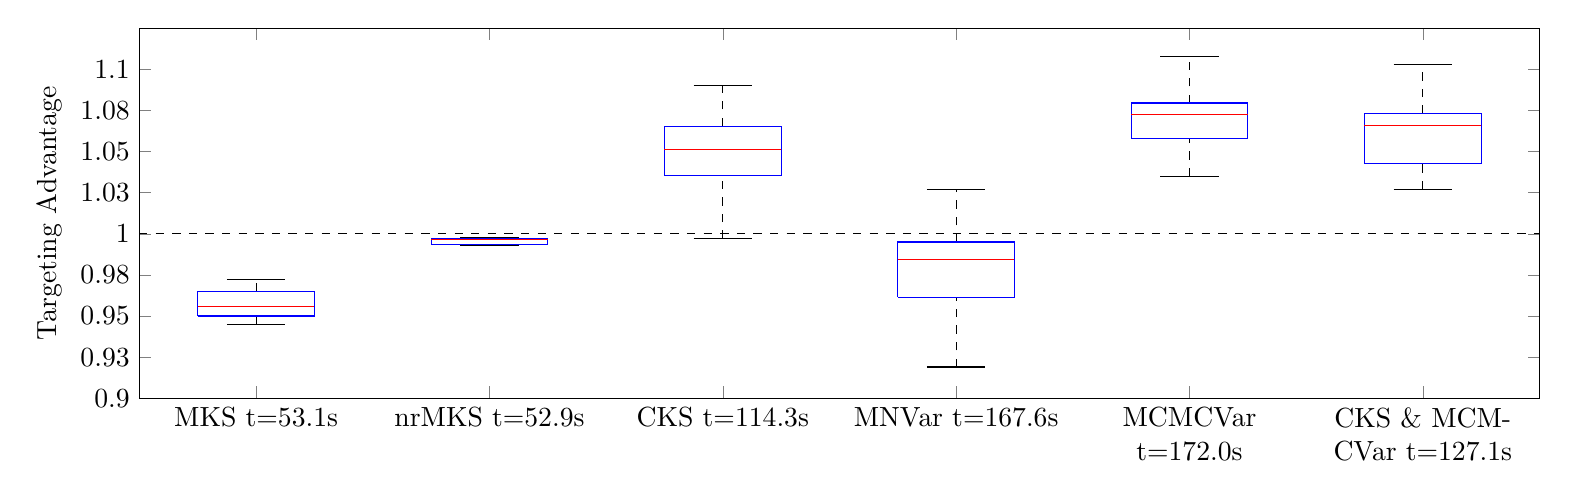
\begin{tikzpicture}

\begin{axis}[%
width=7in,
height=1.85in,
unbounded coords=jump,
scale only axis,
xmin=0.5,
xmax=6.5,
xtick={1, 2, 3, 4, 5, 6,7},%ugliness here
xticklabels={MKS t=53.1s,nrMKS t=52.9s,CKS t=114.3s,MNVar t=167.6s,MCMCVar t=172.0s,CKS \& MCMCVar t=127.1s},%and there
x tick label style={text width=3cm,align=center}, %font=\small,
ymin=0.90,
ymax=1.125,
ytick={.9,.925,.95,.975,1,1.025,1.05,1.075,1.1},
ylabel=Targeting Advantage
]
\addplot [color=black,dashed,forget plot]
  table[row sep=crcr]{1	0.965\\
1	0.972\\
};
\addplot [color=black,dashed,forget plot]
  table[row sep=crcr]{2	0.997\\
2	0.998\\
};
\addplot [color=black,dashed,forget plot]
  table[row sep=crcr]{3	1.0655\\
3	1.09\\
};
\addplot [color=black,dashed,forget plot]
  table[row sep=crcr]{4	0.995\\
4	1.027\\
};
\addplot [color=black,dashed,forget plot]
  table[row sep=crcr]{5	1.0795\\
5	1.108\\
};
\addplot [color=black,dashed,forget plot]
  table[row sep=crcr]{6	1.073\\
6	1.103\\
};
\addplot [color=black,dashed,forget plot]
  table[row sep=crcr]{1	0.945\\
1	0.95\\
};
\addplot [color=black,dashed,forget plot]
  table[row sep=crcr]{2	0.993\\
2	0.9935\\
};
\addplot [color=black,dashed,forget plot]
  table[row sep=crcr]{3	0.997\\
3	1.0355\\
};
\addplot [color=black,dashed,forget plot]
  table[row sep=crcr]{4	0.919\\
4	0.9615\\
};
\addplot [color=black,dashed,forget plot]
  table[row sep=crcr]{5	1.035\\
5	1.058\\
};
\addplot [color=black,dashed,forget plot]
  table[row sep=crcr]{6	1.027\\
6	1.0425\\
};
\addplot [color=black,solid,forget plot]
  table[row sep=crcr]{0.875	0.972\\
1.125	0.972\\
};
\addplot [color=black,solid,forget plot]
  table[row sep=crcr]{1.875	0.998\\
2.125	0.998\\
};
\addplot [color=black,solid,forget plot]
  table[row sep=crcr]{2.875	1.09\\
3.125	1.09\\
};
\addplot [color=black,solid,forget plot]
  table[row sep=crcr]{3.875	1.027\\
4.125	1.027\\
};
\addplot [color=black,solid,forget plot]
  table[row sep=crcr]{4.875	1.108\\
5.125	1.108\\
};
\addplot [color=black,solid,forget plot]
  table[row sep=crcr]{5.875	1.103\\
6.125	1.103\\
};
\addplot [color=black,solid,forget plot]
  table[row sep=crcr]{0.875	0.945\\
1.125	0.945\\
};
\addplot [color=black,solid,forget plot]
  table[row sep=crcr]{1.875	0.993\\
2.125	0.993\\
};
\addplot [color=black,solid,forget plot]
  table[row sep=crcr]{2.875	0.997\\
3.125	0.997\\
};
\addplot [color=black,solid,forget plot]
  table[row sep=crcr]{3.875	0.919\\
4.125	0.919\\
};
\addplot [color=black,solid,forget plot]
  table[row sep=crcr]{4.875	1.035\\
5.125	1.035\\
};
\addplot [color=black,solid,forget plot]
  table[row sep=crcr]{5.875	1.027\\
6.125	1.027\\
};
\addplot [color=blue,solid,forget plot]
  table[row sep=crcr]{0.75	0.95\\
0.75	0.965\\
1.25	0.965\\
1.25	0.95\\
0.75	0.95\\
};
\addplot [color=blue,solid,forget plot]
  table[row sep=crcr]{1.75	0.9935\\
1.75	0.997\\
2.25	0.997\\
2.25	0.9935\\
1.75	0.9935\\
};
\addplot [color=blue,solid,forget plot]
  table[row sep=crcr]{2.75	1.0355\\
2.75	1.0655\\
3.25	1.0655\\
3.25	1.0355\\
2.75	1.0355\\
};
\addplot [color=blue,solid,forget plot]
  table[row sep=crcr]{3.75	0.9615\\
3.75	0.995\\
4.25	0.995\\
4.25	0.9615\\
3.75	0.9615\\
};
\addplot [color=blue,solid,forget plot]
  table[row sep=crcr]{4.75	1.058\\
4.75	1.0795\\
5.25	1.0795\\
5.25	1.058\\
4.75	1.058\\
};
\addplot [color=blue,solid,forget plot]
  table[row sep=crcr]{5.75	1.0425\\
5.75	1.073\\
6.25	1.073\\
6.25	1.0425\\
5.75	1.0425\\
};
\addplot [color=red,solid,forget plot]
  table[row sep=crcr]{0.75	0.956\\
1.25	0.956\\
};
\addplot [color=red,solid,forget plot]
  table[row sep=crcr]{1.75	0.9965\\
2.25	0.9965\\
};
\addplot [color=red,solid,forget plot]
  table[row sep=crcr]{2.75	1.051\\
3.25	1.051\\
};
\addplot [color=red,solid,forget plot]
  table[row sep=crcr]{3.75	0.9845\\
4.25	0.9845\\
};
\addplot [color=red,solid,forget plot]
  table[row sep=crcr]{4.75	1.0725\\
5.25	1.0725\\
};
\addplot [color=red,solid,forget plot]
  table[row sep=crcr]{5.75	1.066\\
6.25	1.066\\
};
\addplot [color=black,dashed,forget plot]
  table[row sep=crcr]{0	1\\
1	1\\
2	1\\
3	1\\
4	1\\
5	1\\
6	1\\
7	1\\
};
\end{axis}
\end{tikzpicture}%}
  \end{center}

  
  \begin{tabular}{p{2.2cm}p{5cm}p{2.2cm}p{5cm}}
  \textbf{MKS:} & Minimum Knowledge Search & \textbf{nrMKS:} & non random MKS \\
  \textbf{CKS:} & Clustered Knowledge Search & \textbf{MNVar:} & Matrix Normal Variance Search \\
  \textbf{MCMCVar:} & Markov Chain Monte Carlo Variance Search & \textbf{CKS \& MCMCvar:} & CKS combined with MCMCVar calculated at 50 sample intervals
  \end{tabular}
  
    Box plot for 20 simulations of active sampling with offline PMF.
  
  t is the time taken for one run of 500 new sample requests.
  
  Values larger than 1 indicate better than random performance.
  
  Lookahead sampling was ignored for computational efficiency reasons.
  
    \caption{Comparison of multiple runs on $80 \times 50$ synthetic data}
    \label{fig:combined_compared}
\end{figure}

Here the performance of all the encountered algorithms so far is evaluated. For fair comparisons it was compared to the average random sampling performance rather than an individual instance(average of random sampling for $80 \times 50$ is found in appendix figure \ref{fig:RandomPMF}). This avoid instances of bad random sampling performance and very good targeted sampling performance creating artificially high values, as in figure \ref{fig:online_pmf_active}.

The first observation to be made is that the proposed MKS algorithm does not perform well, only ensuring close to expected random performance, the non random variation was found to slightly outperform the random variation due to the initial column and row knowledge maximisation (as seen in the knowledge matrix in figure \ref{fig:know_mat_it}).

The CKS search did yield better than random performance nearly consistently, which shows that the targeted approach was successful, though not as well as the more complex MCMCVar one.

Matrix Normal Variance Search (MNVar) did not results in the results found by Sutherland et. al, however this is most likely due to MNVar being sensitive to the parameters used and the parameters found by PMF do not complete empty rows and cells, meaning parameter quality can be very low at the start of the sampling process.

MCMCVar was found to perform best, consistently outdoing random selection, though at the cost of greater complexity. An attempt at reducing complexity while retaining targeting performance is done with the hybrid CKS MCMC algorithm. This resulted in a performance consistently above random sampling and was above to reduce the runtime of 500 sample requests by 27\%. While not very useful for small matrices, as active sampling rarely needs to be done in realtime, this is useful for very large databases such as the Netflix one.


Finally the Max-Min value search mentioned in section \ref{sec:as_goals} was tested but had an average targeting advantage of 0.8 and was only found to be useful to remove some over and under estimation errors, as expected.
% ------------------------------------------------------------------------


%%% Local Variables: 
%%% mode: latex
%%% TeX-master: "../thesis"
%%% End: 
